\chapter[Soluções Adotadas]{Soluções Adotadas}

\subsection{Capta\c{c}\~ao de \'aguas pluviais}

	No Brasil, o sistema para capta\c{c}\~ao de \'agua \'e utilizado em algumas cidades do Nordeste como fonte de suprimento devido aos per\'iodos de seca. A viabilidade do uso de \'agua da chuva \'e caracterizada pela diminui\c{c}\~ao da demanda de \'agua fornecida por companhias de saneamento, gerando assim uma economia de custos com a \'agua e redu\c{c}\~ao de reten\c{c}\~ao da mesma em locais que possam causar enchentes. \cite{MAY} 

	Os principais objetivos da capta\c{c}\~ao e aproveitamento das \'aguas da chuva s\~ao: utiliza\c{c}\~ao nos banheiros, tanto na limpeza quanto nas descargas de vasos sanit\'arios; utilizados na irriga\c{c}\~ao dos jardins na \'epoca de seca; evitando ac\'umulo de \'agua em locais com depress\~ao, por captar a \'agua e canaliz\'a-la para um reservat\'orio.
	
	No processo de capta\c{c}\~ao da \'agua s\~ao utilizadas \'areas imperme\'aveis, como por exemplo, os telhados. Este projeto visa a disponibiliza\c{c}\~ao da coleta da \'agua nos telhados dos banheiros, da administra\c{c}\~ao e das torres de seguran\c{c}a. Nos locais que tiver certa inclina\c{c}\~ao, ser\~ao colocadas calhas capazes de canalizar a \'agua e lev\'a-la para os tanques, onde ser\~ao tratadas e enviadas para sua utiliza\c{c}\~ao. \cite{MAY} 
	
	Segundo a Leal \cite{LEAL}, o sistema de aproveitamento da \'agua da chuva funciona da seguinte maneira: a \'agua \'e coletada de \'areas imperme\'aveis e em seguida \'e filtrada e armazenada em um reservat\'orio de acumula\c{c}\~ao, que pode ser apoiado, enterrado ou elevado e pode ser constru\'ido de diferentes materiais como: concreto armado, bloco de concreto, alvenaria de tijolos, a\c{c}o, pl\'astico, poli\'ester, polietileno e outros.

	Os par\^ametros principais envolvidos no sistema de coleta e aproveitamento da \'agua de chuva s\~ao: \'area de coleta, quantidade de \'agua a ser armazenada, qualidade da \'agua, capacidade de armazenamento e confiabilidade.

	Para n\~ao ocorrerem entupimentos nos dutos que levam a \'agua canalizada para os tanques s\~ao usadas peneiras para retirada de folhas e galhos maiores, essas grades ser\~ao posicionadas por toda a calha aumentando um pouco o custo, por\'em evitando poss\'iveis problemas na filtragem, como pode ser observado na figura abaixo. Ser\~ao usado 122 mm x 3m dessa calha, e pode ser encontrada na Leroy Merlin a um valor de R\$ 59,90. 

\begin{figure}[H]
	\centering
	\label{Grades usadas na calha}
		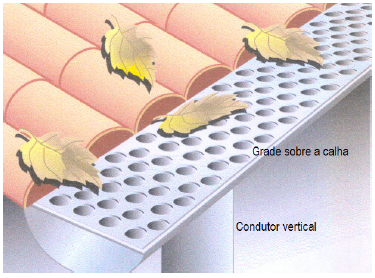
\includegraphics[keepaspectratio=true,scale=0.9]{figuras/GradesUsadasNaCalha.png}
	\caption{Grades usadas na calha}
	\small{Fonte: \cite{WATERFALL} }
\end{figure}

Os condutores, que servem para canalizar a \'agua do telhado ser\~ao as calhas com grades colocadas nas extremidades das constru\c{c}\~oes, como ilustra a Figura abaixo.

\begin{figure}[H]
	\centering
	\label{Sistema de calhas na \'area do telhado}
		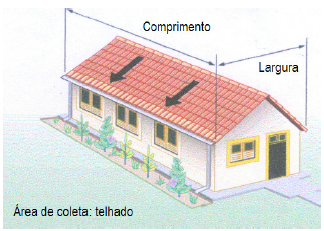
\includegraphics[keepaspectratio=true,scale=1.2]{figuras/SistemaDeCalhasNaAreaDoTelhado.png}
	\caption{Sistema de calhas na \'area do telhado}
	\small{Fonte:  \cite{WATERFALL}}
\end{figure}

O armazenamento ser\'a feito a partir do estudo de 8 tipos de tanques, devido a disponibilidade e a facilidade de constru\c{c}\~ao, para tanto foi realizado um estudo, apresentado na figura abaixo, da capacidade de armazenamento, viabilidade econ\^omica, e m\~ao-de-obra.

\begin{figure}[H]
	\centering
	\label{TipoDeTanques}
		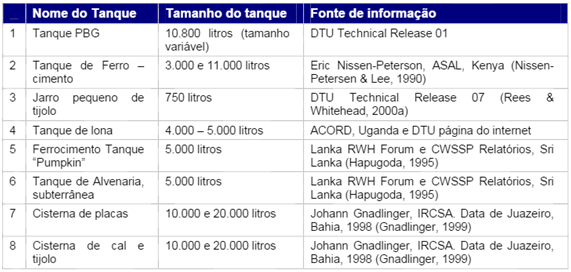
\includegraphics[keepaspectratio=true,scale=1.0]{figuras/TipoDeTanques.png}
	\caption{Tipo de Tanques}
	\small{Fonte:  \cite{TERRYTHOMAS}}
\end{figure}

\begin{figure}[H]
	\centering
	\label{ComparativoDosTanques}
		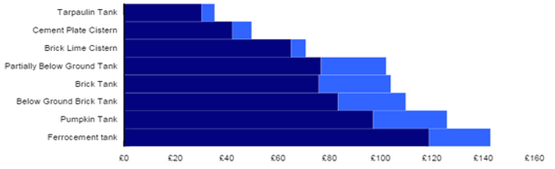
\includegraphics[keepaspectratio=true,scale=1.2]{figuras/ComparativoDosTanques.png}
	\caption{Comparativo dos Tanques}
	\small{Fonte:  \cite{TERRYTHOMAS}}
\end{figure}

 Esse gr\'afico, apresentado na figura acima, foi feito a partir da figura \ref{TipoDeTanques} acima sobre os tipos de tanques, mostrando o custo do material, a convers\~ao foi feita seguindo a cota\c{c}\~ao atual, sendo 1 libra esterlina igual a 4,36 reais.
 
 	Tendo em vista os tanques estudados na figura \ref{ComparativoDosTanques} , o que se mostrou mais economicamente atrativo foi o \textit{Cement Plate Cistern} , a cisterna de placas cimentadas, a qual armazena de 10 mil a 20 mil litros de \'agua, o mesmo \'e melhor para o parque devido ao seu custo de opera\c{c}\~ao e instala\c{c}\~ao serem baixos, o cimento \'e barato, gerando um custo de 500 reais para a constru\c{c}\~ao. O tanque do tipo placas cimentadas segue a ideia de ser encostado na edifica\c{c}\~ao, portanto eles ser\~ao posicionados ao lado dos banheiros, guarita de seguran\c{c}a, administra\c{c}\~ao e quiosque sem consumir muito espa\c{c}o e com sinaliza\c{c}\~ao para que os usu\'arios n\~ao mexam na instala\c{c}\~ao. A Figura a seguir apresenta o sistema de capta\c{c}\~ao de \'agua a ser implantado no Parque do Gama.\cite{JOHANN} 
 
 \begin{figure}[H]
	\centering
	\label{SistemaDeCaptacao}
		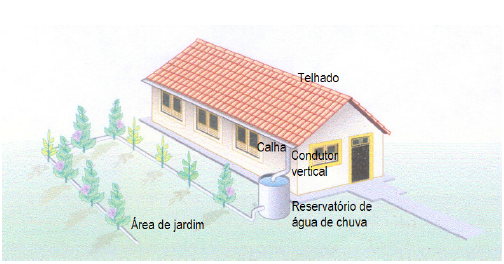
\includegraphics[keepaspectratio=true,scale=1.0]{figuras/SistemaDeCaptacao.png}
	\caption{Sistema de capta\c{c}\~ao}
	\small{Fonte:  \cite{WATERFALL}}
\end{figure}
 
 A figura abaixo mostra a quantidade de litros de \'agua em uma irriga\c{c}\~ao de acordo com o di\^ametro da mangueira, mostrando a quantidade de \'agua p\'ublica que \'e perdida com essa atividade. Sendo assim, ser\'a utilizada uma mangueira de $^{3}$/$_{4}$ polegadas por apresentar maior vaz\~ao volum\'etrica.  Por exemplo, para um uso de 15 minutos, seriam gastos 499 litros de \'agua, portanto seria aconselh\'avel o reuso da \'agua de chuva para tal atividade.
 
 \begin{figure}[H]
	\centering
	\label{ConsumoAguaRega}
		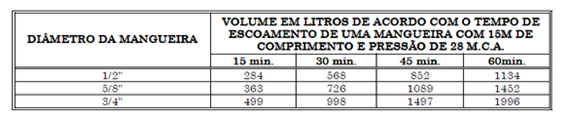
\includegraphics[keepaspectratio=true,scale=1.0]{figuras/ConsumoAguaRega.png}
	\caption{Estimativa do consumo da \'agua na torneira de jardins por tempo de rega}
	\small{Fonte:  \cite{VICKERS}}
\end{figure}
 
Um ponto relevante a ser considerado \'e que em hip\'otese alguma a \'agua da chuva captada poder\'a ser misturada a \'agua pot\'avel. Al\'em disso, \'e necess\'ario que ocorra a limpeza da \'agua. Para isso, ser\'a usado um filtro VF1 o qual recebe a \'agua da chuva e filtra os galhos e folhas que passaram pela grade das calhas, em seguida, a \'agua passa por uma tela de malha de 0,26 mm que se localiza abaixo das ripas e \'e direcionada ao reservat\'orio. A frequ\^encia da manuten\c{c}\~ao varia conforme a incid\^encia da sujeira, ocorrendo de 1 a 2 vezes ao ano. O filtro \'e mostrado abaixo e pode ser encontrado no valor de 2100 reais. \cite{VICKERS} 
 
\begin{figure}[H]
	\centering
	\label{SistemaDeFiltroUtilizado}
		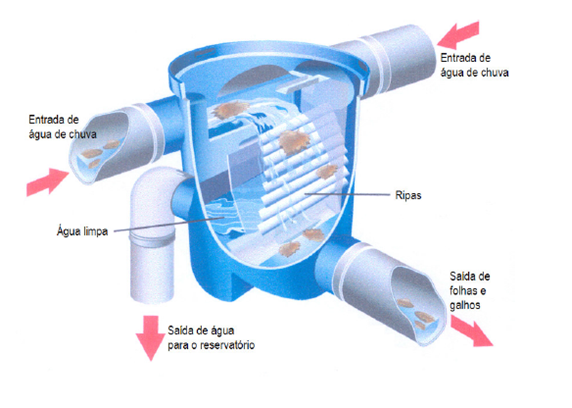
\includegraphics[keepaspectratio=true,scale=0.8]{figuras/SistemaDeFiltroUtilizado.png}
	\caption{Sistema de filtro utilizado}
	\small{Fonte:  \cite{TECHINIK}}
\end{figure}
 
A figura a seguir apresenta o tipo da \'agua da chuva, com o filtro usado e a desinfec\c{c}\~ao requerida. No parque ser\'a utilizada \'agua n\~ao pot\'avel, pois apresenta filtros e tratamento qu\'imico com cloro, para no caso de contato com a pele, n\~ao cause nenhum efeito colateral.
 
\begin{figure}[H]
	\centering
	\label{TipoAguaPropriedadesExigidas}
		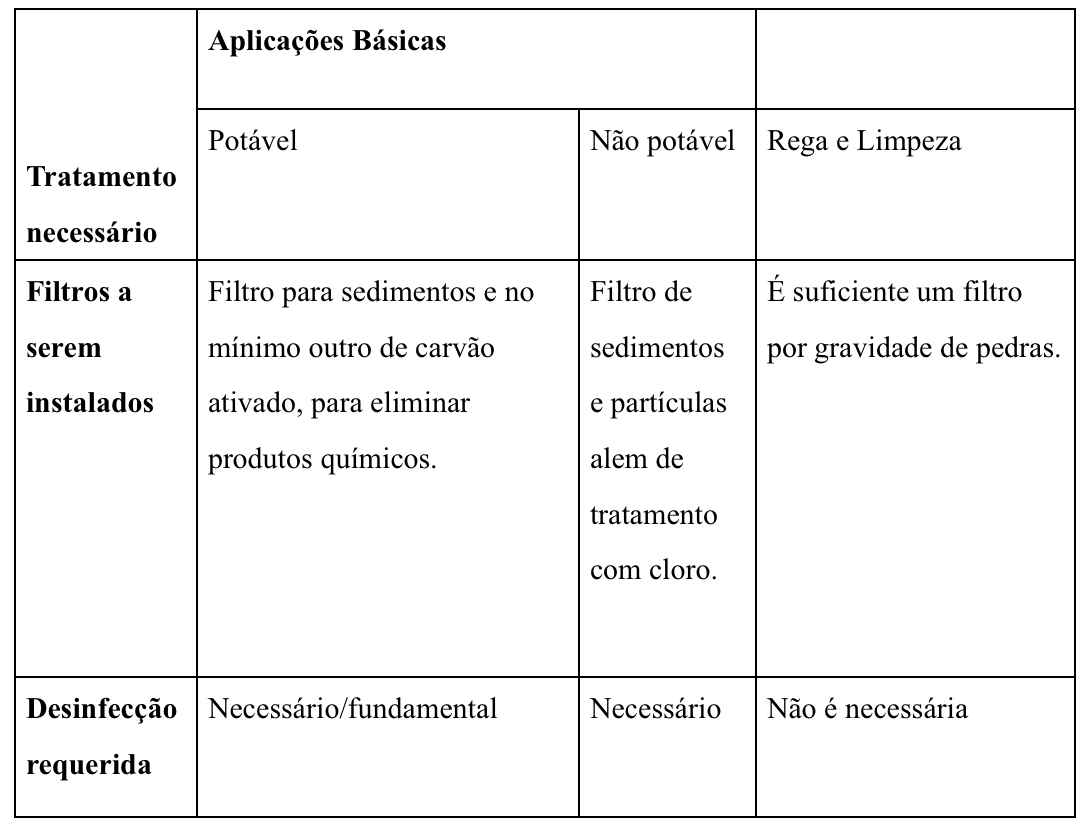
\includegraphics[keepaspectratio=true,scale=0.8]{figuras/TipoAguaPropriedadesExigidas.png}
	\caption{Tipo da \'agua e propriedades exigidas}
\end{figure}
 
  A qualidade da \'agua \'e definida pela sua composi\c{c}\~ao f\'isica, qu\'imica e bacteriol\'ogica. Como a \'agua pluvial captada n\~ao ser\'a direcionada para o consumo ela n\~ao precisa ser pot\'avel. Portanto, o tratamento necess\'ario \'e um cuidado com bact\'erias ou qualquer organismo capaz de provocar enfermidades. \cite{MINISTERIODASAUDE} Mesmo a \'agua n\~ao sendo utilizada para o consumo ela deve ser corretamente tratada por entrar em contato com os seres humanos na irriga\c{c}\~ao, nas descargas do banheiro ou na limpeza, n\~ao podendo, ent\~ao, conter bact\'erias que possam prejudicar a sa\'ude de algum visitador do parque.
  
	A desinfec\c{c}\~ao de \'agua de chuva poder\'a ser realizada atrav\'es de sistema simples, como atrav\'es de adi\c{c}\~ao de cloro, para n\~ao inviabilizar economicamente o sistema. O cloro dever\'a ser aplicado de forma mais homog\^enea poss\'ivel, devendo repetir a opera\c{c}\~ao sempre que o teor de cloro ficar muito baixo alem de n\~ao alterar no pH da \'agua. O pre\c{c}o do cloro \'e relativamente baixo, de em torno de 150 reais o pote de 10kg.
	
	Para bombeamento da \'agua ser\'a utilizado uma bomba com uso de painel solar Shurflo 8000 com o valor de 800 reais que bombeia at\'e 1700L de \'agua por dia a uma altura de 42m, sendo mais que suficiente para trazer a \'agua captada para ser usada. Portanto, ela \'e auto suficiente por captar energia solar at\'e com pequena irradia\c{c}\~ao solar com placa de 140Wp.
	
	O sistema de capta\c{c}\~ao de \'agua reduzir\'a notavelmente o consumo total de \'agua do parque, e nos per\'iodos de seca. Essa \'agua armazenada poder\'a ser devidamente utilizada para irriga\c{c}\~ao dos jardins pr\'oximos \`a \'area do banheiro, al\'em de servir para o uso em descargas e limpeza dos pisos. O reuso da \'agua da chuva que ser\'a instalado \'e um \'otimo caminho para tornar o parque em um parque modelo de sustentabilidade.
	
	Dessa forma, o custo de constru\c{c}\~ao girar\'a em torno de 4300 reais por local de instala\c{c}\~ao, contando com a m\~ao de obra e com os materiais. Para a manuten\c{c}\~ao foi estipulado um valor de 200 reais por m\^es para m\~ao de obra e purifica\c{c}\~ao da \'agua, assim em aproximadamente um ano a \'agua economizada com a instala\c{c}\~ao desse sistema de capta\c{c}\~ao cobrir\'a os custos iniciais, levando em considera\c{c}\~ao a quantidade de pessoas que frequentar\~ao o parque e a quantidade de chuvas que pode variar a cada ano.
  
\subsection{Plano de Cercamento}

Cada vez mais a marginalidade inserida na sociedade tem afetado pessoas de todas as classes sociais sem distin\c{c}\~ao de ra\c{c}a, sexo ou posi\c{c}\~ao social. A necessidade de prover de um ambiente protegido \'e uma das exig\^encias b\'asicas para que a popula\c{c}\~ao possa frequentar o parque urbano do gama em um momento de lazer. Com base em entrevistas realizadas com a popula\c{c}\~ao local notou-se que se faz necess\'ario um novo projeto de cercamento, pois a falta de cercamento pode provocar uma inseguran\c{c}a aos frequentadores do parque e uma facilidade de acesso em qualquer localidade do parque, o que dificulta o controle de acesso de pessoas que tem como consequ\^encia uma poss\'ivel pr\'atica de vandalismo e mau uso dos recursos do parque.

	Esse projeto prop\~oem um planejamento de cercamento do parque urbano do gama, especificando os materiais, dimens\~oes e tipo de cerca que ser\'a usada para o cercamento com base em normas t\'ecnicas usadas para esse tipo de atividade. O cliente ter\'a dispon\'ivel de todo passo a passo e especifica\c{c}\~oes t\'ecnicas para a correta instala\c{c}\~ao do cercamento. Esse projeto n\~ao ir\'a identificar as partes do cercamento que ainda est\~ao em condi\c{c}\~oes de uso ou que poder\~ao ser reutilizadas, cabendo ao interessado contratar um especialista para a verifica\c{c}\~ao do mesmo.
	
	Ser\'a reformado o cercamento em um per\'imetro de 3342,29 metros (Documento anexo x1 vivencial do gama geral) e adicionado uma nova cerca nos per\'imetros onde n\~ao houver como recuperar a cerca danificada.Tanto os materiais quanto as especifica\c{c}\~oes t\'ecnicas utilizadas para o cercamento do parque urbano do gama ser\~ao os da empresa Metalgrade, que possui certifica\c{c}\~ao de qualidade NBR ISO 9001 e \'e adequada para esse tipo de obra.  O tipo de cerca utilizada ser\'a o gradil eletrofundido \textit{Stadium} que \'e composto estruturalmente por arames redondos verticais e horizontais formando malhas retangulares enrijecidas por dobras trapezoidais horizontais, configurando-se um design moderno e singular. O conjunto \'e complementado com  pilares parafusados (com sapata). \cite{CatalogoCercamento} \\ O esquema a seguir mostra as especifica\c{c}\~oes t\'ecnicas e dimens\~oes do gradil eletrofundido \textit{Stadium} com pilar chumbado:

\begin{figure}[H]
	\centering
	\label{EspecificacoesTecnicasCerca}
		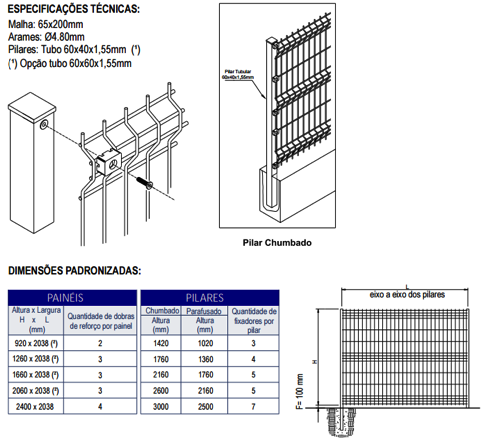
\includegraphics[keepaspectratio=true,scale=0.8]{figuras/EspecificacoesTecnicasCerca.png}
	\caption{Especifica\c{c}\~oes t\'ecnicas para a montagem da cerca.}
	\small{Fonte: \cite{CatalogoCercamento}}
\end{figure}

O passo a passo a seguir mostra detalhadamente cada etapa do procedimento de instala\c{c}\~ao do gradil, que deve ser seguindo \`a risca para que n\~ao haja nem um tipo de problema no cercamento posteriormente \`a instala\c{c}\~ao da grade: 

\textbf{1$^{o}$ Passo: Funda\c{c}\~ao} \\ Primeiro deve-se delimitar o alinhamento e fazer a funda\c{c}\~ao de acordo com o tamanho do eixo do gradil escolhido com 200mm e profundidade de 500mm

\begin{figure}[H]
	\centering
	\label{GradilEscolhido}
		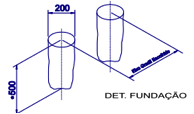
\includegraphics[keepaspectratio=true,scale=0.9]{figuras/GradilEscolhido.png}
	\caption{Passo 1, funda\c{c}\~ao para o gradil escolhido.}
	\small{Fonte: \cite{CatalogoCercamento}}
\end{figure}

\textbf{2$^{o}$ Passo: Pr\'e montagem} \\ Neste segundo passo deve-se fazer a  pr\'e montagem dos pain\'eis e posteriormente posicion\'a-los em p\'e e apoi\'a-los.

\begin{figure}[H]
	\centering
	\label{MontagemPaineisPilares}
		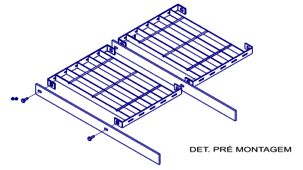
\includegraphics[keepaspectratio=true,scale=0.8]{figuras/MontagemPaineisPilares.png}
	\caption{Passo 2, montagem dos pain\'eis e pilares.}
	\small{Fonte: \cite{CatalogoCercamento}}
\end{figure}

\textbf{3$^{o}$ Passo: Montagem sequencial} \\ Neste passo deve-se pegar os demais pain\'eis e ir montando seguindo o passo anterior(passo 2) e assim ate o termino da montagem.

\begin{figure}[H]
	\centering
	\label{MontagemSequencialPaineis}
		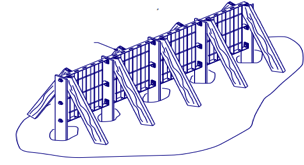
\includegraphics[keepaspectratio=true,scale=0.8]{figuras/MontagemSequencialPaineis.png}
	\caption{Passo 3, montagem sequencial de todos pain\'eis.}
	\small{Fonte:  \cite{CatalogoCercamento}}
\end{figure}

\textbf{4$^{o}$ Passo: Aprumar e alinhar} \\ Nesta etapa deve-se estender as linhas superior e inferior entre o primeiro e o ultimo painel para alinhar o conjunto, ajustando as escoras para conservar o alinhamento.

\textbf{5$^{o}$ Passo: Concretagem} \\ Neste \'ultimo passo deve-se concretar as bases da cerca e mant\^e-las escoradas por no m\'inimo 24 horas.

\begin{figure}[H]
	\centering
	\label{ConcretagemBasesPilares}
		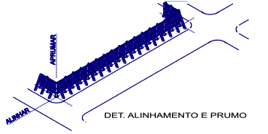
\includegraphics[keepaspectratio=true,scale=0.8]{figuras/ConcretagemBasesPilares.png}
	\caption{Passo 5, concretagem das bases dos pilares.}
	\small{Fonte: \cite{CatalogoCercamento}}
\end{figure}

\subsection{Relat\'orio de Pain\'eis Solares}

\subsubsection{Comparativos das tecnologias dos sistemas fotovoltaicos}

Um sistema fotovoltaico \'e normalmente classificado em \textbf{Sistema Isolado}  (n\~ao conectado a rede el\'etrica da concession\'aria) ou \textbf{Sistema Conectado}  (conectado a rede el\'etrica da concession\'aria) e \'e usual mente constitu\'ido por:

 \begin{itemize}
        \item Painel fotovoltaico
	\item Regulador de Carga		(para sistemas isolados)
	\item Inversor
	\item Baterias	(para sistemas isolados)
\end{itemize}

Os sistemas existentes s\~ao os seguintes:

\begin{itemize}
        \item Sistemas isolados dom\'esticos (\textit{Off-grid domestic}): sistemas que fornecem energia el\'etrica para ilumina\c{c}\~ao, refrigera\c{c}\~ao e outras pequenas cargas em locais isolados. 
	\item Sistemas isolados n\~ao dom\'esticos (\textit{Off-grid non-domestic}): sistemas que fornecem energia el\'etrica a servi\c{c}os, tais como, telecomunica\c{c}\~oes, bombeamento de \'agua, frigor\'ificos m\'edicos, ajuda \`a navega\c{c}\~ao a\'erea e mar\'itima, esta\c{c}\~oes de recolha de dados meteorol\'ogicos.
	\item Sistemas distribu\'idos conectados \`a rede (\textit{Grid-connected distributed}): sistemas que fornecem energia el\'etrica a edif\'icios (comerciais ou industriais) ou outras cargas que tamb\'em est\~ao ligadas \`a rede, para onde a energia em excesso \'e enviada. A pot\^encia t\'ipica para este tipo de aplica\c{c}\~oes varia entre 0,5 kW e 100 kW.
	\item Sistemas centralizados conectados \`a rede (\textit{Grid-connected centralized}): sistemas que fornecem exclusivamente energia el\'etrica \`a rede.
\end{itemize}

\subsubsection{Sistemas isolados}

Os sistemas isolados ou aut\^onomos para gera\c{c}\~ao de energia solar fotovoltaica s\~ao caracterizados por n\~ao se conectarem a rede el\'etrica. O sistema abastece diretamente os aparelhos que utilizar\~ao a energia e s\~ao geralmente constru\'idos com um prop\'osito, local e espec\'ifico. Esta solu\c{c}\~ao \'e muito utilizada em locais remotos, j\'a que muitas vezes \'e o modo mais econ\^omico e pr\'atico de se obter energia el\'etrica nestes locais.

	Os sistemas isolados de gera\c{c}\~ao de energia solar fotovoltaica, de maneira simplificada, s\~ao compostos de quatro componentes:

 \begin{itemize}
        \item \textbf{Pain\'eis solares ou placas solares:} s\~ao eles que geram a energia el\'etrica que abastece as baterias. Tem a propriedade de transformar a radia\c{c}\~ao solar em corrente el\'etrica cont\'inua. Um sistema pode ter apenas um painel ou v\'arios pain\'eis interligados entre si.
	\item \textbf{Controladores de carga:} garantem o correto abastecimento das baterias evitando sobrecargas e aumentando sua vida \'util.
	\item \textbf{Inversores:} s\~ao o c\'erebro do sistema e tem a fun\c{c}\~ao de transformar corrente continua (CC) em corrente alternada (AC), e levar a tens\~ao, por exemplo, de 12V para 127V. Em alguns casos pode ser ligado a outro tipo de gerador ou \`a pr\'opria rede el\'etrica para abastecer as baterias.
	\item \textbf{Baterias:} s\~ao os reservat\'orios do sistema e armazenam a energia el\'etrica para ser utilizada nos momentos em que o sol n\~ao esteja presente e n\~ao haja outras fontes de energia.
\end{itemize}

\subsubsection{Sistemas conectados a rede}

Em aplica\c{c}\~oes ligadas \`a rede de energia el\'etrica, o gerador fotovoltaico entrega \`a rede a m\'axima pot\^encia que, em cada instante, pode produzir. Entre o m\'odulo e a rede existem equipamentos de regula\c{c}\~ao e interface que otimizam as condi\c{c}\~oes de gera\c{c}\~ao e as adaptam \`as condi\c{c}\~oes de recep\c{c}\~ao impostas pela rede. Em termos esquem\'aticos, a situa\c{c}\~ao pode ser descrita como se ilustra na figura abaixo.

\begin{figure}[H]
	\centering
	\label{SistemaFotovoltaico}
		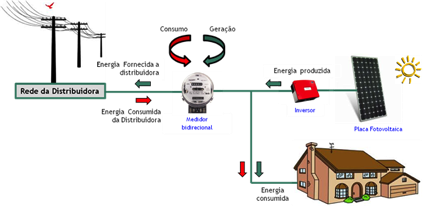
\includegraphics[keepaspectratio=true,scale=0.8]{figuras/SistemaFotovoltaico.png}
	\caption{Esquema de um sistema fotovoltaico ligado \`a rede}
	\small{Fonte:  \cite{Viridian}}
\end{figure}

Do ponto de vista dos componentes, um sistema fotovoltaico conectado \`a rede \'e similar ao sistema isolado com a diferen\c{c}a que o sistema conectado n\~ao necessita de baterias para armazenamento de energia.\\ 

Para a utiliza\c{c}\~ao no Parque Vivencial e Urban\'istico do Gama, n\~ao h\'a a necessidade de se instalar um sistema isolado, que \'e mais caro. Portanto o Sistema Conectado \`a rede \'e mais vi\'avel.

\subsubsection{An\'alise do Projeto}

A partir das plantas do projeto foi estimado um valor de consumo el\'etrico, usando uma simula\c{c}\~ao, para as seguintes edifica\c{c}\~oes:

 \begin{itemize}
        \item Sede Administrativa
	\item Guaritas
	\item Quiosques
	\item Banheiros
\end{itemize}

\begin{itemize}
      \item Sede Administrativa
             \begin{itemize}
                       \item \'Area \'util para placa solar	=	59,032 m$^{2}$ 
                       \item Consumo el\'etrico estimado	=	787,37 kWh 
	     \end{itemize}
\end{itemize}

\begin{figure}[H]
	 \centering
	 \label{SistemaGeradorSede}
	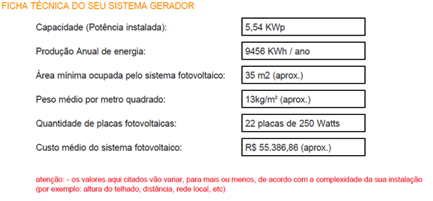
\includegraphics[keepaspectratio=true,scale=0.8]{figuras/SistemaGeradorSede.png}
	\caption{Ficha t\'ecnica do sistema gerador da Sede Administrativa}
	\small{Fonte: \cite{PortalSolar}}
\end{figure}

\begin{itemize}
         \item Banheiro (x2)
	           \begin{itemize}
                       \item \'Area \'util para placa solar	=	21,824 m$^{2}$ 
                       \item Consumo el\'etrico estimado	=	89,88 kWh 
                  \end{itemize}	 
\end{itemize}

\begin{figure}[H]
	  \centering
	 \label{SistemaGeradorBanheiro}
	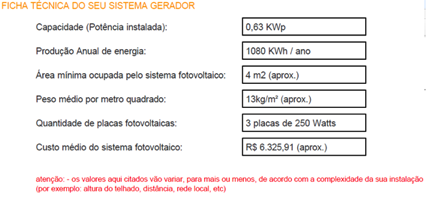
\includegraphics[keepaspectratio=true,scale=0.8]{figuras/SistemaGeradorBanheiro.png}
	\caption{Ficha t\'ecnica do sistema gerador do banheiro}
	\small{Fonte: \cite{PortalSolar}}
\end{figure}

\begin{itemize}
         \item Guarita (x2)
	           \begin{itemize}
                       \item \'Area \'util para placa solar	=	8,41 m$^{2}$ 
                       \item Consumo el\'etrico estimado	=	77,62 kWh  
                  \end{itemize}	
\end{itemize} 

 \begin{figure}[H]
	\centering
	\label{SistemaGeradorGuarita}
	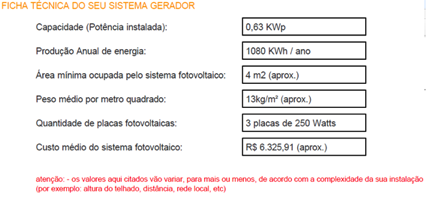
\includegraphics[keepaspectratio=true,scale=0.8]{figuras/SistemaGeradorBanheiro.png}
	\caption{Ficha t\'ecnica do sistema gerador da Guarita}
	\small{Fonte: \cite{PortalSolar}}
\end{figure}

\begin{itemize}
         \item Quiosque (x2)
	           \begin{itemize}
                       \item \'Area \'util para placa solar	=	25 m$^{2}$ 
                       \item Consumo el\'etrico estimado	=	466,10 kWh      
                  \end{itemize}	 
\end{itemize}

\begin{figure}[H]
	 \centering
	\label{SistemaGeradorQuiosque}
	 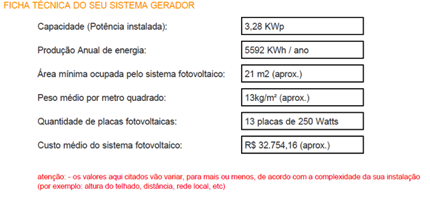
\includegraphics[keepaspectratio=true,scale=0.8]{figuras/SistemaGeradorQuiosque.png}
	 \caption{Ficha t\'ecnica do sistema gerador do Quiosque}
	\small{Fonte: \cite{PortalSolar}}
\end{figure}

Total

 \begin{itemize}
        \item \'Area \'util para placa solar	=	169,5 m$^{2}$ 
        \item \'Area necess\'aria	=	93 m$^{2}$ 
        \item Consumo el\'etrico estimado	=	2054,57 kWh
	\item Quantidade de placas necess\'arias	=	60 (de 250 W)
	\item Custo do sistema + instala\c{c}\~ao	=	144.511,92 reais
\end{itemize}

\subsection{Projeto de ilumina\c{c}\~ao}

\subsubsection{Defini\c{c}\~oes de Termos Luminot\'ecnicos}

Para uma maior compreens\~ao do projeto ser\'a abordado alguns termos luminot\'ecnicos e el\'etricos necess\'arios para a compreens\~ao das demais se\c{c}\~oes. De acordo com o manual de ilumina\c{c}\~ao p\'ublica da COPEL, temos:

 \begin{itemize}
        \item Fluxo Luminoso - O fluxo luminoso pode ser entendido como a quantidade de energia radiante em todas as dire\c{c}\~oes, emitida por unidade de tempo, e avaliada de acordo com a sensa\c{c}\~ao luminosa produzida. A unidade de medida \'e o l\'umen (lm).
	\item Efici\^encia Luminosa - A efici\^encia luminosa \'e a rela\c{c}\~ao entre o fluxo luminoso emitido pela pot\^encia el\'etrica absorvida, sendo a unidade de medida o l\'umen por \textit{watt} (lm/W). Este conceito \'e utilizado para comparar a diferentes fontes luminosas.
	\item Iluminamento ou ilumin\^ancia - ilumin\^ancia \'e a densidade de fluxo luminoso recebido por uma superf\'icie. Por defini\c{c}\~ao a unidade de medida \'e o l\'umen por metro ao quadrado (lm/m$^{2}$), que pode ser denominada tamb\'em de lux. A verifica\c{c}\~ao deste par\^ametro \'e fundamental para comprovar a qualidade da ilumina\c{c}\~ao de um determinado local.
	\item Fator de uniformidade - O fator de uniformidade \'e uma rela\c{c}\~ao entre a ilumin\^ancia m\'inima e a m\'edia de uma determinada \'area. Resulta em um valor adimensional variando entre zero e a unidade, que indica como est\'a a distribui\c{c}\~ao da luminosidade na superf\'icie aferida. Umin = Emed/Emin (Manual de Ilumina\c{c}\~ao P\'ublica fevereiro de 2012 SED/DNGO/VNOT P\'agina 4)
	\item Temperatura de cor - Este par\^ametro n\~ao est\'a relacionado com o calor emitido por uma l\^ampada, mas pela sensa\c{c}\~ao de conforto que a mesma proporciona em um determinado ambiente. Quanto mais alto for o valor da temperatura de cor, mais branca ser\'a a luz emitida, denominada comumente de "luz fria" e que \'e utilizada, por exemplo, em ambientes de trabalho, pois induz maior atividade ao ser humano. No entanto, caso seja baixa a temperatura de cor, a luz ser\'a mais amarelada, proporcionando uma maior sensa\c{c}\~ao de conforto e relaxamento, chamada popularmente de "luz quente", utilizada preferencialmente em salas de estar ou quartos. As fontes luminosas artificiais podem variar entre 2000K (muito quente) at\'e mais de 10000K (muito fria).
	\item \'Indice de reprodu\c{c}\~ao de cor - O \'indice de reprodu\c{c}\~ao de cor (IRC) de uma fonte luminosa \'e a medida de cor real de uma superf\'icie e sua apar\^encia a ser iluminada pela fonte artificial. Uma fonte com IRC 100\% \'e a que apresenta as cores de um objeto com a m\'axima fidelidade. Na figura abaixo, \'e apresentado o mesmo local sob as mesmas condi\c{c}\~oes, por\'em iluminado com fontes luminosas diferentes. \`a esquerda a ilumina\c{c}\~ao \'e feita por \textit{LED's} (light emitting diode ou diodo emissor de luz) de alto IRC, e \`a direita com l\^ampadas a vapor de s\'odio em alta press\~ao com baixo IRC. Nota-se que na segunda situa\c{c}\~ao a defini\c{c}\~ao das cores \'e prejudicada.
\end{itemize}

\begin{figure}[H]
	 \centering
	\label{ComparativoDuasFontesLuminosas}
	 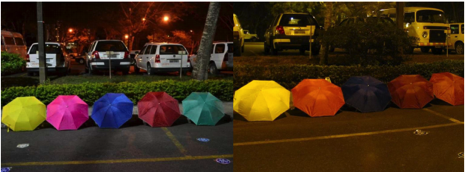
\includegraphics[keepaspectratio=true,scale=0.8]{figuras/ComparativoDuasFontesLuminosas.png}
	 \caption{Comparativo entre duas fontes luminosas com diferentes IRC's}
	\small{Fonte: \cite{COPELPARANA} }
\end{figure}

\begin{itemize}
        \item Vida mediana- Tempo ap\'os o qual 50\% das l\^ampadas de uma determinada amostragem, submetidas a um ensaio de vida, deixam de funcionar.
	\item Distor\c{c}\~ao harm\^onica total - Entende-se por distor\c{c}\~ao harm\^onica total (THDi - \textit{Total Harmonic Distortion}), a rela\c{c}\~ao entre a soma dos valores eficazes de todas as componentes harm\^onicas de uma determinada forma de onda pelo valor eficaz de sua componente fundamental, expresso normalmente em termos percentuais. Para este manual, define-se THDi como a distor\c{c}\~ao harm\^onica da corrente absorvida por uma carga n\~ao linear, em geral equipamentos eletroeletr\^onicos, em rela\c{c}\~ao \`a onda senoidal pura com frequ\^encia de 60Hz, fornecida pela concession\'aria. Com relativa intensidade, uma corrente com elevado THDi pode provocar distor\c{c}\~oes nas formas de onda da corrente e tens\~ao do sistema el\'etrico, reduzindo a qualidade da energia entregue e prejudicando o funcionamento de outros equipamentos conectados \`a mesma rede.  \cite{COPELPARANA}
\end{itemize}

\begin{figure}[H]
	 \centering
	\label{FormulaTHDI}
	 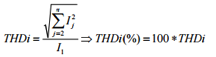
\includegraphics[keepaspectratio=true,scale=0.8]{figuras/FormulaTHDI.png}
	 \caption{F\'ormula THDi}
\end{figure}

Em que: \\ I$_{j}$ \'e o valor eficaz da componente harm\^onica da corrente absorvida pela carga \textit{e}. \\ I$_{1}$ \'e a componente fundamental da corrente, com frequ\^encia de 60Hz. \\ THDi(\%) \'e a distor\c{c}\~ao harm\^onica total da corrente expressa em valores percentuais.

\begin{itemize}
        \item Fator de Pot\^encia - O fator de pot\^encia \'e definido pela raz\~ao entre as pot\^encias ativa (P) e aparente (S) de um circuito, resultando em um n\'umero adimensional entre zero e um. Quanto mais pr\'oximo da unidade for o fator de pot\^encia, indica que a energia est\'a sendo consumida de forma mais eficiente, visto que apenas a pot\^encia ativa realiza trabalho efetivamente. No entanto, quanto mais pr\'oximo a zero indica que a maior parte da energia consumida \'e reativa, necess\'aria para o funcionamento de elementos armazenadores de energia, como indutores e capacitores, mas que deve ser compensada, pois gera perdas e diversas perturba\c{c}\~oes no sistema el\'etrico. A equa\c{c}\~ao completa para o c\'alculo do fator de pot\^encia \'e dada por:
\end{itemize}

\begin{figure}[H]
	 \centering
	\label{FormulaFP}
	 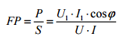
\includegraphics[keepaspectratio=true,scale=0.8]{figuras/FormulaFP.png}
	 \caption{F\'ormula FP}
\end{figure}

Onde: U$_{1}$ e I$_{1}$ s\~ao os valores eficazes das componentes fundamentais da tens\~ao e corrente, respectivamente, de um circuito \\
U e I s\~ao os valores eficazes totais da tens\~ao e corrente, respectivamente, calculados da seguinte forma:

\begin{figure}[H]
	 \centering
	\label{FormulaX}
	 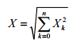
\includegraphics[keepaspectratio=true,scale=0.8]{figuras/FormulaX.png}
	 \caption{F\'ormula X}
\end{figure}

Em que: X$_{k}$ \'e o valor eficaz da componente harm\^onica que comp\~oe a forma de onda.
cos $\phi$ \'e o co-seno do \^angulo $\phi$ de desfasamento entre a corrente e a tens\~ao. \cite{COPELPARANA}

	Na maioria dos casos, as tens\~oes e correntes do sistema el\'etrico podem ser consideradas senoidais puras, logo seus valores eficazes totais s\~ao iguais aos de suas componentes fundamentais. Assim a equa\c{c}\~ao para o c\'alculo do fator de pot\^encia se resume ao co-seno do \^angulo $\phi$: FP = cos$\phi$
	
	No entanto, h\'a situa\c{c}\~oes no sistema el\'etrico em que as tens\~oes e correntes n\~ao s\~ao senoidais puras. Para estes casos a equa\c{c}\~ao geral para o c\'alculo do fator de pot\^encia deve ser utilizada. Para o c\'alculo do fator de pot\^encia dos equipamentos abrangidos por este manual, deve-se utilizar a equa\c{c}\~ao apresentada na sequ\^encia, que \'e resultado da inser\c{c}\~ao do conceito da total distor\c{c}\~ao harm\^onica da corrente apresentada na Distor\c{c}\~ao Harm\^onica Total. Na equa\c{c}\~ao geral, desprezando as poss\'iveis distor\c{c}\~oes na forma de onda da tens\~ao. Observa-se que, caso a corrente absorvida pela carga seja senoidal pura, o valor de THDi ser\'a nulo, e o resultado da equa\c{c}\~ao ser\'a apenas o co-seno do \^angulo de desfasamento entre a tens\~ao e a corrente.

\begin{figure}[H]
	 \centering
	\label{FormulaFP2}
	 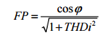
\includegraphics[keepaspectratio=true,scale=0.8]{figuras/FormulaFP2.png}
	 \caption{F\'ormula FP utilizando THDi}
\end{figure}

\subsubsection{Projeto de Ilumina\c{c}\~ao P\'ublica de \'Areas para Pedestres}

A ilumina\c{c}\~ao p\'ublica nas \'areas utilizadas predominantemente por pedestres deve prover seguran\c{c}a, conforto e a capacidade de reconhecer os eventos ao seu redor a uma dist\^ancia razo\'avel. \cite{CemigMinas}

\subsubsection{Ilumina\c{c}\~ao de Pra\c{c}as e Parques}

Nas cidades, as pra\c{c}as e parques contribuem n\~ao s\'o para o embelezamento, mas tamb\'em promovem o lazer, recrea\c{c}\~ao e o conv\'ivio entre as pessoas. Dessa forma, uma aten\c{c}\~ao especial deve ser dada na elabora\c{c}\~ao dos projetos de ilumina\c{c}\~ao destes espa\c{c}os p\'ublicos, no sentido de torn\'a-los seguros e convidativos \`a comunidade. Contudo, a ilumina\c{c}\~ao \'e apenas um dos muitos componentes respons\'aveis pela melhoria do ambiente urbano. Sempre que necess\'ario, deve-se promover uma reforma nas condi\c{c}\~oes desses espa\c{c}os p\'ublicos.\cite{CemigMinas}

	Algumas pra\c{c}as ou parques, em fun\c{c}\~ao de sua concep\c{c}\~ao arquitet\^onica, apresentam \'areas distintas de utiliza\c{c}\~ao como jardins, brinquedos, jogos de mesa, quadras, etc. Nestes casos, podem ser aplicados crit\'erios de projetos diferenciados para cada espa\c{c}o. Efeitos atrativos podem ser criados pelo uso de l\^ampadas com temperatura de cor diferente. Por exemplo, se utilizarmos l\^ampadas VS para a ilumina\c{c}\~ao do entorno, o interior da pra\c{c}a pode ser iluminada com l\^ampadas VMT.\cite{CemigMinas}
	
	A ilumina\c{c}\~ao de escadas e rampas para acesso dos pedestres deve ser ponto de aten\c{c}\~ao e considerados na loca\c{c}\~ao dos postes de forma que estas mudan\c{c}as de n\'ivel sejam bem vis\'iveis. Est\'atuas, \'arvores, coretos e outros pontos de interesse especial, podem ser individualmente iluminados. Postes com altura de montagem superior a 5 metros somente devem ser instalados em pra\c{c}as e cal\c{c}ad\~oes onde \'e poss\'ivel o acesso dos ve\'iculos de manuten\c{c}\~ao. Esta restri\c{c}\~ao vale tamb\'em para os espa\c{c}os onde o piso n\~ao estiver adequado ao peso destes ve\'iculos. Se uma pra\c{c}a possuir pequenas dimens\~oes, a melhoria da ilumina\c{c}\~ao das vias do entorno pode evitar a instala\c{c}\~ao de um projeto espec\'ifico. Nos cal\c{c}ad\~oes, a disposi\c{c}\~ao da ilumina\c{c}\~ao n\~ao deve obstruir o acesso dos ve\'iculos de emerg\^encia ou de manuten\c{c}\~ao. \cite{CemigMinas} 

\subsubsection{N\'iveis de iilumin\^ancia e uniformidade}

A ilumina\c{c}\~ao destes espa\c{c}os deve permitir no m\'inimo um reconhecimento m\'utuo, al\'em de proporcionar informa\c{c}\~ao visual suficiente a respeito das pessoas e suas inten\c{c}\~oes a uma dist\^ancia segura. Segundo estudos realizados, a dist\^ancia m\'inima necess\'aria para uma pessoa reconhecer qualquer sinal de hostilidade e tomar as a\c{c}\~oes evasivas apropriadas \'e de 4 metros. A esta dist\^ancia, o n\'ivel de ilumin\^ancia m\'edio m\'inimo necess\'ario para reconhecimento facial \'e de 5 lux. De toda forma, sobre a superf\'icie n\~ao deve haver valor inferior a 1 lux. Considerando a necessidade de identifica\c{c}\~ao de obst\'aculos na superf\'icie da via e a velocidade com que as pessoas ou eventualmente ciclistas trafegam, o fator de uniformidade (U) n\~ao deve ser inferior a 0,25. A Tabela 2 apresenta as recomenda\c{c}\~oes para o n\'ivel de ilumin\^ancia m\'edia e informa o valor m\'inimo para o fator de uniformidade para cada classe de ilumina\c{c}\~ao de pedestres. \cite{CemigMinas}

\subsubsection{Ciclovia e ciclofaixa}

Considerando a import\^ancia crescente das bicicletas como meio de transporte nas cidades, a ilumina\c{c}\~ao das ciclovias contribui para a redu\c{c}\~ao dos acidentes o que \'e particularmente importante quando existem cruzamentos com vias de tr\^ansito de ve\'iculos automotores. Os principais requisitos de visibilidade a serem fornecidos pela ilumina\c{c}\~ao s\~ao:

\begin{itemize}
        \item As altera\c{c}\~oes no trajeto e os limites da ciclovia e ciclofaixa; 
        \item A presen\c{c}a de obst\'aculos fixos na superf\'icie, tais como mobili\'ario urbano, \'arvores, etc;
	\item A visualiza\c{c}\~ao de buracos e rachaduras na superf\'icie da pista;
	\item A posi\c{c}\~ao e a velocidade dos usu\'arios da ciclovia;
	\item A exist\^encia de cruzamentos com as vias que conduzem outro tipo de tr\'afego;
\end{itemize}

As lumin\'arias utilizadas devem ser instaladas com espa\c{c}amentos m\'inimos de 3,5 vezes a altura de montagem. Para a maioria das ciclovias e ciclofaixas, os requisitos para a escolha da fonte de luz devem considerar os crit\'erios utilizados para a ilumina\c{c}\~ao das demais vias urbanas como vida mediana, rendimento. Contudo, pode ser necess\'ario utilizar uma l\^ampada de cor diferente da existente na via adjacente a fim de chamar a aten\c{c}\~ao dos motoristas quanto \`a exist\^encia da ciclovia ou ciclofaixa. A tabela abaixo apresenta as recomenda\c{c}\~oes para o n\'ivel de ilumin\^ancia m\'edia e informa o valor m\'inimo para o fator de uniformidade para ciclovias e ciclofaixas. Conforme a NBR 5101:1992 temos os limites fotom\'etricos para vias de trafego de pedestres segundo a tabela abaixo. \cite{COPELPARANA} 

\begin{table}[H]
\caption{Limites fotom\'etricos para vias de tr\'afego motorizado e de pedestres} 
\begin{center}
\begin{tabular}{|p{8cm}|p{4cm}|p{4cm}|} \hline

Descri\c{c}\~ao da Via &E$_{m\'in}$ (lux) &U$_{m\'in}$ \\ \hline 

Vias de uso noturno intenso por pedestres (por exemplo, cal\c{c}ad\~oes, passeios de zonas comerciais) &20 &0,3 \\ \hline
Vias de grande tr\'afego noturno de pedestres (por exemplo, passeios de avenidas, pra\c{c}as, \'areas de lazer) &10 &0,25 \\ \hline
Vias de uso noturno moderado por pedestres (por exemplo, passeios, acostamentos) &5 &0,2 \\ \hline
Vias de pouco uso por pedestres (por exemplo, passeios de bairros residenciais) &3 &0,2 \\ \hline
Circuito da ciclovia ou ciclofaixa &5 &0,3 \\ \hline
Cruzamento de vias com trafego motorizado &10 &0,3 \\ \hline

 \end{tabular}
\end{center}
\end{table}

\subsubsection{\'Areas de Ilumina\c{c}\~ao}

De acordo com os padr\~oes de ilumina\c{c}\~ao p\'ublica estabelecidos pelas normas brasileiras, para manter o n\'ivel de m\'inimo de ilumina\c{c}\~ao ou ilumin\^ancia, obteve-se o seguinte padr\~ao de posicionamento dos poste de acordo com a figura abaixo:

\begin{figure}[H]
	 \centering
	\label{PosicionamentoPostes}
	 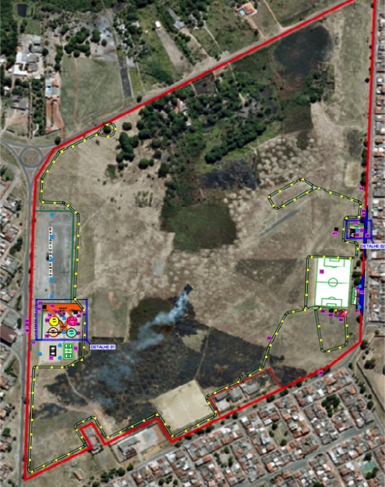
\includegraphics[keepaspectratio=true,scale=0.8]{figuras/PosicionamentoPostes.png}
	 \caption{Padr\~ao de posicionamento dos postes}
	 \small{Fonte: Google, 2015}
\end{figure}

Os pontos amarelos que est\~ao situados na ciclovia s\~ao os postes do modelo PTS 305/315 que distam aproximadamente 27 metros entre si, totalizando 103 postes ao longo de toda a ciclovia. Segue na  figura 2 abaixo as especifica\c{c}\~oes t\'ecnicas desse modelo:

\begin{figure}[H]
	 \centering
	\label{PTS305}
	 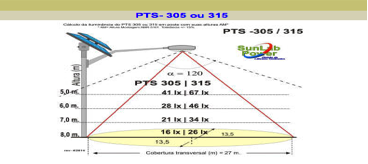
\includegraphics[keepaspectratio=true,scale=0.8]{figuras/PTS305.png}
	 \caption{Especifica\c{c}\~oes t\'ecnicas poste PTS - 305/315}
	 \small{Fonte: \cite{SUNLABPTS}}
\end{figure}

J\'a os pontos azuis que est\~ao situados nas \'areas de conviv\^encia social, s\~ao os postes do modelo PTS 405/410. Na \'area designada a um dos estacionamentos foram alocados 5 postes que distam entre si aproximadamente 30 metros, e no restante das \'areas de conviv\^encia social foram alocados postes de acordo com a necessidade, totalizando 13 postes desse modelo. Segue na figura 3 abaixo as especifica\c{c}\~oes t\'ecnicas desse modelo:

\begin{figure}[H]
	 \centering
	\label{PTS405}
	 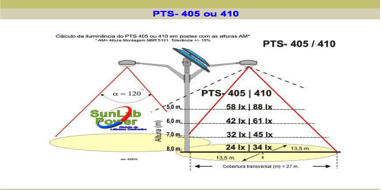
\includegraphics[keepaspectratio=true,scale=0.8]{figuras/PTS405.png}
	 \caption{Especifica\c{c}\~oes t\'ecnicas poste PTS - 405/410}
	 \small{Fonte: \cite{SUNLABPTS}}
\end{figure}

É importante atentar que o futuro campo de futebol a direita da imagem j\'a \'e iluminado, n\~ao sendo vi\'avel sua remo\c{c}\~ao, j\'a que os mesmos s\~ao espec\'ificos para campos e \'areas grandes que necessitam de bastante ilumina\c{c}\~ao, por\'em a esquerda no estacionamento, haver\'a a trocas dos postes existentes para os escolhidos neste ponto de controle, a substitui\c{c}\~ao dos mesmos acarretar\'a em uma economia de energia a longo prazo e o desvinculamento com a rede da CEB, padronizando assim a sua manuten\c{c}\~ao.

	A tabela abaixo mostra os padr\~oes de luminot\'ecnicos dos postes avaliados e dos postes dos respectivos PTS - 305/315 e PTS - 405/10 que ser\~ao usados na revitaliza\c{c}\~ao do parque, os dois modelos escolhidos foram os que melhor se enquadraram nos padr\~oes de ilumina\c{c}\~ao segundo os manuais de ilumina\c{c}\~ao da companhias energ\'eticas dos estados da federa\c{c}\~ao:

\begin{figure}[H]
	 \centering
	\label{TabelaModelosPoste}
	 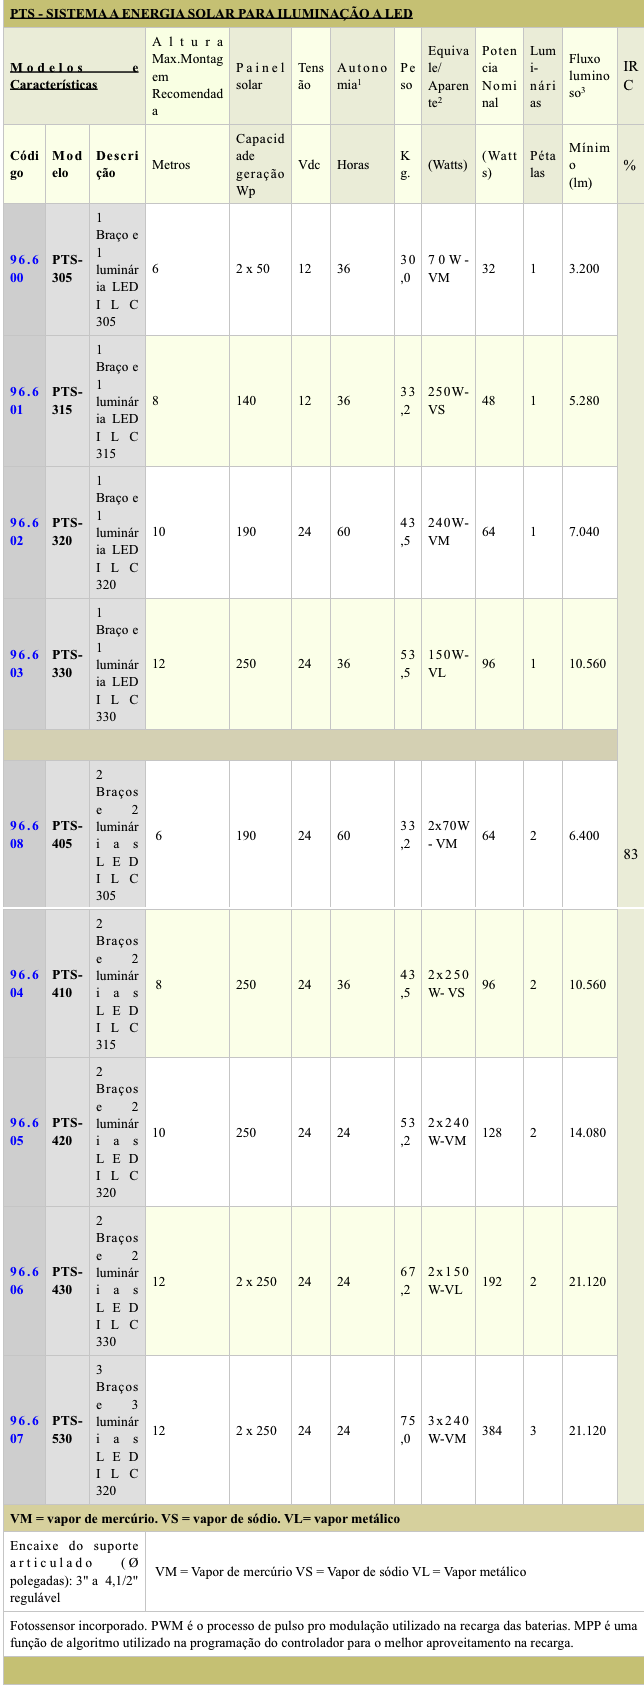
\includegraphics[keepaspectratio=true,scale=0.4]{figuras/TabelaModelosPoste.png}
	 \caption{Modelos de postes da linha PTS}
\end{figure}

\subsection{Interação social e atratividade do parque}

	A partir da problemática apresentada, a falta de atratividade do parque, o grupo de Interação Social definiu a orientação das soluções no sentido mais material, ou seja, no sentido de dar a estrutura necessária para que a futura administração do parque possa promover eventos e atividades educacionais com recursos tecnológicos.

	Fomentar a edução de jovens e crianças, promover atividades físicas à toda população próxima ao parque (desde jovens até o público idoso) foram as motivações que impulsionaram o grupo a pensar em soluções práticas, de custo acessível e disponível gratuitamente a toda a população do Gama.

	Sendo assim, todas as soluções estão integradas e promovendo a interação da comunidade afim de tornar as atividades de lazer contínuas e bem definidas.
	
	Primeiramente identificou-se a necessidade de um espaço para eventos e realizações de atividades recreativas como por exemplo:

\begin{itemize}
	\item Aulas de ginástica para jovens e idosos;
	\item Cinema comunitário e eventos de promoção ao lazer e cultura;
	\item Aulas temáticas para crianças e jovens, incentivando conhecimentos ambientais, regionais e que promovam os cursos da Faculdade UnB Gama (FGA) por exemplo;
	\item Eventos comunitários como festas comemorativas, assembléias de moradores, reuniões de grupos sociais e filantrópicos, entre outras utilidades. Esses eventos poderiam ser agendados gratuitamente na administração do parque;
\end{itemize}

	Todo esse ambiente social e de interação entre a comunidade do parque estaria reunido em um aplicativo para \textit{smartphones} e \textit{tablets}, onde os frequentadores do parque interagiriam com o ambiente com as pessoas que o frequentam, obteriam informações relevantes sobre o parque, sua construção, ambiente e curiosidades, bem como informações sobre eventos e sobre os outros frequentadores.

	Sendo um incentivo ao uso da tecnologia, o parque do gama atende a todas as preocupações dos usuários, portanto o parque contará com tomadas e carregadores de celular acessíveis ao público, nos locais de vivencia social.

	Haja vista toda essa gama de possibilidades de boas soluções para o parque, o grupo procurou adequar o projeto inicial, que já esta em implementação pela administração do Gama, às novas necessidades tecnológicas verificadas.

\subsubsection{Espaço interativo e vivência}

	Após discussões e análises em busca de uma primazia para o parque do Gama, chegou-se a uma dedução no que se refere ao fascínio por parte da população ao parque: Criação de um espaço multimídia.
Os elementos que compõem o escopo para que essa atratividade seja atingida são; Aulas interativas para a população, que contará com sistemas de áudio e video de alta tecnologia, gerando assim uma experiência única de aprendizagem. Práticas de exercícios físicos para a população com um viés de sustentabilidade, que será alcançado com aulas de spinning em bicicletas que gerarão energia elétrica. E para complementar, também serão realizados espetáculos e solenidades com o auxilio das tecnologias já mencionadas.

	Para que essas atividades sejam realizadas, uma estrutura física deverá ser erguida em formato de tenda, que terá um tamanho de 2.000 $m^{2}$, as figuras 1.1 e 1.2 mostram uma perspectiva da futura instalação. Esse espaço será constituído por uma estrutura metálica e por uma cobertura em PVC. A estrutura será fabricada em tubos de metalon de aço carbono com pontos soldados eletricamente em MIG e intervalado por parafusos com porca auto-travante, essa estrutura ficará em uma área fixa do parque, e com os devidos cuidados informados pelo fabricante deve possuir uma vida útil extremamente longa.
A cobertura em PVC será vulcanizada com sistema de termo fixação eletrônica, evitando-se assim o uso de costuras. A cobertura será em vinil VINISET que será impermeável, resistente a rasgos, bloqueador solar para melhor sensação térmica, auto-extinguível (não se propaga fogo), anti-fungo e anti-oxidante. Um dos pontos negativos em relação a cobertura será a sua durabilidade, a qual devido as condições naturais do tempo, possuem sua vida útil em torno de cinco anos.

	A inclinação para a escolha desse tipo de estrutura e não para as estruturas convencionais, como as de alvenaria, se deve ao fato do projeto ter como foco, o baixo custo. A única estrutura feita em alvenaria colocada e representada na figura abaixo, será o dep\'osito dos equipamentos do espaço, pois estes possuem alto valor e requerem uma maior segurança para que não sejam furtados. A conclusão do projeto, segundo empresas especializadas no segmento, terá como intervalo de tempo 90 dias, dentro desse tempo contará a criação e aprovação do projeto por engenheiro responsável.
	
\begin{figure}[H]
	 \centering
	\label{Tenda Modelo Padrão}
	 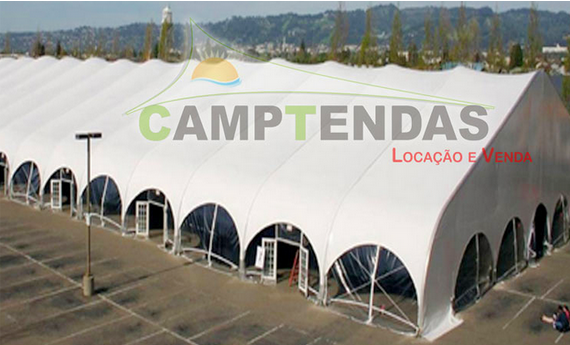
\includegraphics[keepaspectratio=true,scale=0.8]{figuras/TendaModeloGalpao.png}
	 \caption{Tenda Modelo Galpão}
	 \small{Fonte: camptendas.com.br}
\end{figure}

\begin{figure}[H]
	 \centering
	\label{Visão Interna Tenda}
	 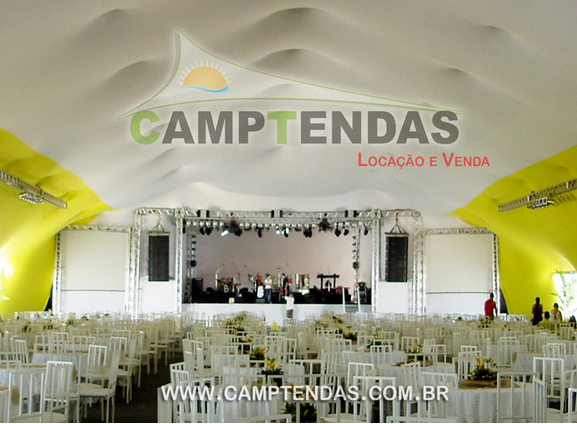
\includegraphics[keepaspectratio=true,scale=0.8]{figuras/VisaoInternaTenda.png}
	 \caption{Visão Interna da Tenda}
	 \small{Fonte: camptendas.com.br}
\end{figure}

\begin{figure}[H]
	 \centering
	\label{Deposito Dos Equipamentos}
	 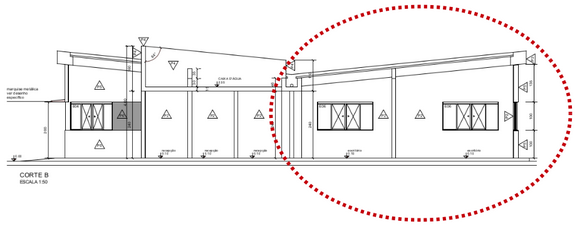
\includegraphics[keepaspectratio=true,scale=0.8]{figuras/DepositoDosEquipamentos.png}
	 \caption{Deposito dos equipamentos do espaço interativo}
	 \small{Fonte: Fornecida pela Administração Regional do Gama-DF}
\end{figure}

\subsubsection{Locais permitidos para construção no Parque Vivencial do Gama}

	Dentro do Parque do Gama existem nascentes que restringem qualquer construção em um raio de 50 (cinquenta) metros das mesmas, de acordo com a Lei Federal 4.771/65, alterada pela Lei 7.803/89 e a Medida Provisória nº 2.166-67, de 24 de agosto de 2001, “Consideram-se de preservação permanente, pelo efeito de Lei, as áreas situadas nas nascentes, ainda que intermitentes e nos chamados ‘olhos d’água’, qualquer que seja a situação topográfica, devendo ter um raio mínimo de 50 (cinquenta) metros de largura”. 

	A área imediatamente circundante à nascente, em um raio de 50 (cinquenta) metros, é só e exclusivamente uma área de preservação permanente. A restrição para se fazer uso dessa área existe para evitar que, com um cultivo, por exemplo, a nascente fique sujeita à erosão e que as atividades agrícolas de preparo do solo, adubação, plantio, cultivos, colheita e transporte dos produtos levem trabalhadores, máquinas e animais de tração para o local, contaminando física, biológica e quimicamente a água.

	A área adjacente à nascente deve ser toda cercada a fim de evitar o acesso de animais, pessoas, veículos, etc. Todas as medidas devem ser tomadas para favorecer seu isolamento, tais como proibir a pesca e a caça, evitando-se a contaminação do terreno ou diretamente da água por indivíduos inescrupulosos. Quando da realização de alguma obra ou serviço temporário, devem-se construir fossas secas a 30 (trinta) metros, no mínimo, mantendo-se uma vigilância constante para não haver poluição da área circundante à nascente.

	Pode-se localizar na imagem abaixo as nascentes no Parque Vivencial do Gama, de acordo com o texto contendo informações técnicas do parque cedido pela Administração Regional do Gama – RA II, e com isso ter o embasamento de áreas que são permitidas fazer qualquer construção ou alteração.
	
\begin{figure}[H]
	 \centering
	\label{Regiões das nascentes e vederedas}
	 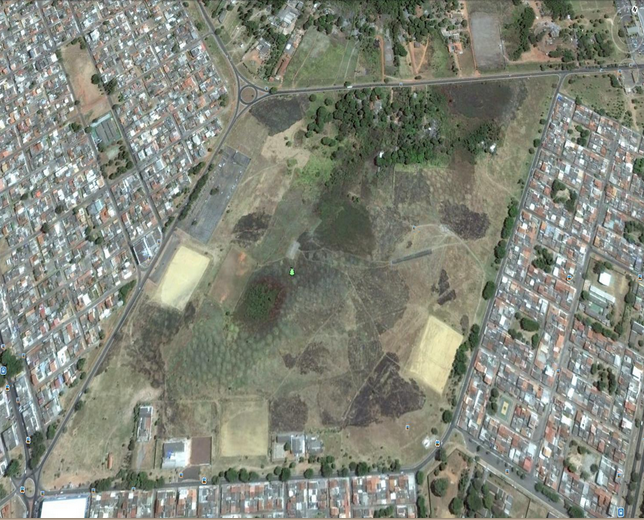
\includegraphics[keepaspectratio=true,scale=0.8]{figuras/RegioesDasNascentes.png}
	 \caption{Regiões acinzentadas são regiões de nascentes e veredas}
	 \small{Fonte: Google Earth, 2015}
\end{figure}

	No mapa abaixo está marcado onde será o espaço desenvolvido para os eventos no parque, o local fica próximo ao estacionamento. O motivo da escolha foi a facilidade e praticidade que as pessoas terão em encontrar e chegar ao local.

\begin{figure}[H]
	 \centering
	\label{Localização do espaço de eventos}
	 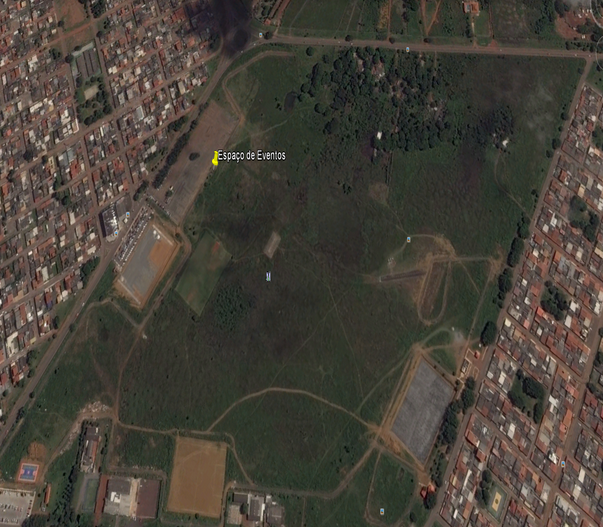
\includegraphics[keepaspectratio=true,scale=0.8]{figuras/LocalEspacoEvento.png}
	 \caption{Localização do Espaço de eventos}
	 \small{Fonte: Google Earth}
\end{figure}

\subsubsection{Sistemas de aulas de ginástica com bicicletas ergométricas sustentável}

	A idéia deste projeto é gerar energia elétrica de uma forma limpa, segura e sustentável, a partir da transformação de energia mecânica cinética, utilizando bicicletas ergométricas, em energia elétrica, que ficarão localizadas dentro do espaço  interativo e serão utilizadas para aulas de spinning com a comunidade do Gama, utilizando os telões e o sistema de sonorização para fazer a interação da aula e motivar os moradores a frequentar as aulas.

	Com base em um projeto de cinema ao ar livre e festivais de música em Londres, surgiu a idéia de adaptar as bicicletas em geradores para que toda energia transformada, seja enviada a uma estação de energia para ser utilizada como alimento para grandes telões, equipamentos de som. A idéia é muito promissora e deve ser aceita pela comunidade frequentadora do parque. É uma maneira sustentável que conta com a ajuda da comunidade para ter um ótimo funcionamento.
	
	Esse sistema de cinema ao ar livre já é utilizado em Londres, com apenas 30 bicicletas e é possível que 1000 pessoas possam assistir a um filme com a energia gerada. Nosso projeto não será ao ar livre, mas contará com a mesma capacidade. Serão adaptadas 30 bicicletas, em dois tamanhos para facilitar sua utilização a todos os públicos, podendo ter um público máximo de até 1000 pessoas.
	
\begin{figure}[H]
	 \centering
	\label{Funcionamento do Telão por energia gerada por bicicletas}
	 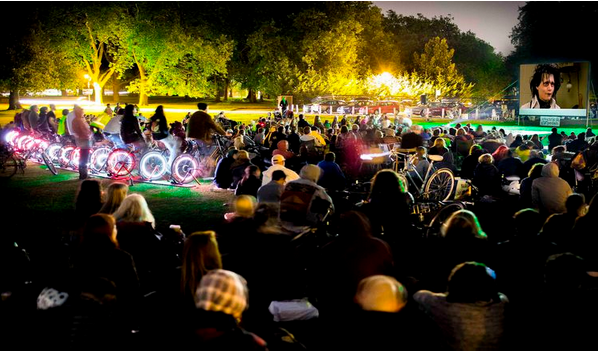
\includegraphics[keepaspectratio=true,scale=0.8]{figuras/TelaoFuncionamentoEnergiaBicicleta.png}
	 \caption{Telão em funcionamento com a energia gerada pelas bicicletas em Londres}
	 \small{Fonte: electricpedals.squarespace.com}
\end{figure}

\begin{figure}[H]
	 \centering
	\label{Evento realizado com as bicicletas}
	 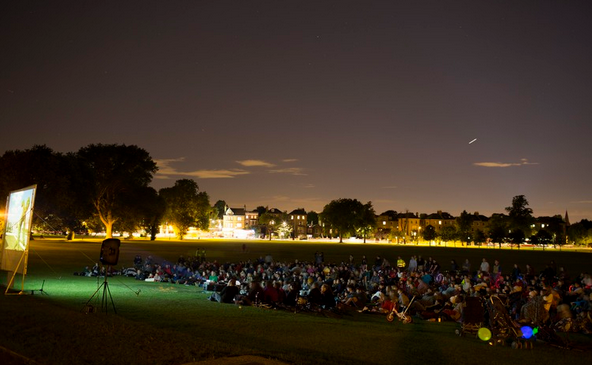
\includegraphics[keepaspectratio=true,scale=0.8]{figuras/TelaoFuncionamentoEnergiaBicicleta2.png}
	 \caption{Evento realizado com as bicicletas}
	 \small{Fonte: electricpedals.squarespace.com}
\end{figure}

\begin{figure}[H]
	 \centering
	\label{Festival de música}
	 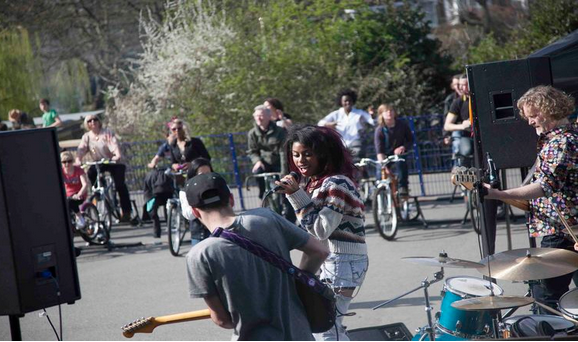
\includegraphics[keepaspectratio=true,scale=0.8]{figuras/TelaoFuncionamentoEnergiaBicicleta3.png}
	 \caption{Festival de música}
	 \small{Fonte: electricpedals.squarespace.com}
\end{figure}

\subsubsection{Produtos}

	Serão utilizadas 20 bicicletas de aro 26, com 18 marchas, e 10 bicicletas de aro 24, com preço aproximado de R\$230,00, com quadro de aço carbono, pesando aproximadamente 14kg, corrente fina, pedal de plástico e com garfo rígido. Serão adaptados em cada bicicletas pneus novos, estilo liso, para uma melhor eficiência. 
	
	Cada bicicleta seria acoplada a um suporte que estará ligado a um gerador, que será tracionado pelo pneu traseiro da bicicleta. O suporte e o gerador serão, baseados nos suporte e geradores da \textit{Eletric Pedals}, que é um projeto feito em Peckham, Londres. Nesse projeto, utiliza-se bicicletas para gerar energia em pequenos eventos, para carregar notebooks, celulares, ligar telas e equipamentos de som onde as pessoas vão pedalando e com suas pedaladas geram energia para tal finalidade.
	
	Outra idéia que será usada como referencia é da \textit{Eletric Pedals}, uma estação de energia (\textit{Power Station Quark}) que administra eficientemente a energia produzida por até 30 pessoas utilizando seus geradores de Energia. Essa estação de energia não possui baterias, usa apenas ultra-capacitores para armazenar e reduzir a energia gerada antes, de fornecer uma segura fonte de alimentação AC 230 volts limpa.

\pagebreak
\begin{itemize}
	\item \textit{Bicycle Friction Generator}: Gerador

	\begin{figure}[H]
	 \centering
	\label{Gerador bicicleta}
	 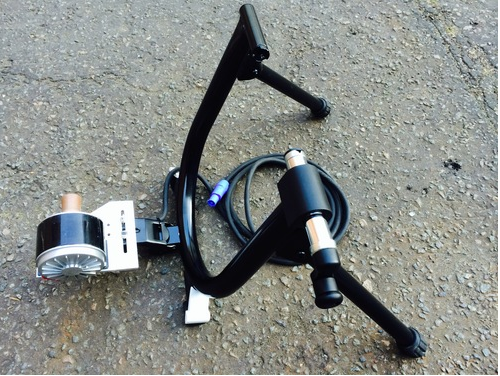
\includegraphics[keepaspectratio=true,scale=0.8]{figuras/bicycle.png}
	 \caption{Gerador no qual a bicicleta é acoplada, projetado para gerar eletricidade usando uma bicicleta padrão.}
	 \small{Fonte: electricpedals.squarespace.com}
	\end{figure}

	\begin{itemize}
	\item Características
	\end{itemize}

		Esse gerador, produz eletricidade regulamentada DC. Fornece um máximo de 400 watts, potência média durante um 	período de tempo geralmente em torno de 40-60 watts por pessoa. Possui 6-8m \textit{Heavy Duty} cabo e conector rápido, bloqueio de diodo. 200 watts 24 volts motor de ímã permanente. Dobras para o armazenamento compacto e um peso de 7,5 Kg.
	
\begin{itemize}
	\item Aplicações
\end{itemize}	
	
	Escolas : Pode ser utilizado para aulas ao ar livre.
Aparelhos domésticos: Aparelhos de baixa potência, como laptops, música , iluminação e carregamento de celular. Mais aparelhos podem ser alimentados, quando combinados com a uma Mini Central Elétrica.
Banco de bateria: Pode ser usado para carregar uma bateria ou um banco de baterias.

\end{itemize}

\begin{itemize}
	\item Capacitor power station quark (Estação de enegia)
	
	Administra a energia produzida por até 30 pessoas que utilizam os geradores. Ele não tem baterias, utiliza alguns super eficiente ultra-capacitores para armazenar e suavizar a energia gerada antes de fornecer a uma fonte segura de AC230 volts limpos.
	\begin{itemize}
		\item Características
		Encerrados em pesados casos de voo, inversor de onda senoidal. Possui uma tensão de saída de 230 V AC (+/-) 2\%. 2000 watts contínuo de potência de saída. Entrada máxima de 200 A para 30 pessoas. Além de possuir componentes reforçados é super eficiente.
	\end{itemize}
	
	\begin{itemize}
		\item Aplicações
		Cinema : Usado em conjunto com qualquer um gerador de energia, pode ser usada para alimentar um cinema ao ar livre para até 1000 pessoas.
Música: Pode em conjunto com um gerador alimentar um pequeno palco de música.
	\end{itemize}
	
	\begin{itemize}
		\item Especificações
		Possui uma saída do inversor de 2000 watts contìnua ( potência de pico de 4000 watts ), tem uma inversão máxima de 92\% de sua eficiência 2000 farad no ultra-capacitor. Uma gestão de tensão com base arduino. 2x251 A de fusíveis. Possui um ponto terra, 10 milímetros de um painel frontal em policarbonato transparente. Dimensões (LxPxA): 1,700 milímetros x 510 milímetros x 500 milímetro e um peso de 60 Kg.
	\end{itemize}
	
	\begin{figure}[H]
	 \centering
	\label{Estação de energia}
	 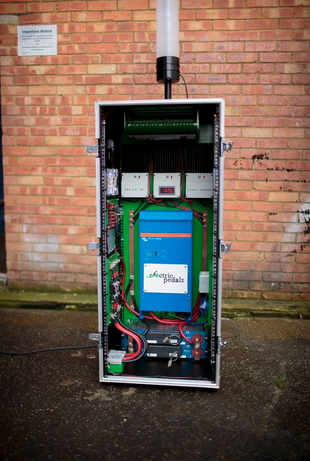
\includegraphics[keepaspectratio=true,scale=0.8]{figuras/capacitor.png}
	 \caption{Power Station Quark (Estação de Energia)}
	 \small{Fonte: electricpedals.squarespace.com}
	\end{figure}	
	
\end{itemize}

\pagebreak
\begin{itemize}
	\item \textit{Bus Board}: Distribuidor
	
	\begin{figure}[H]
	 \centering
	\label{Bus Board: Distribuidor}
	 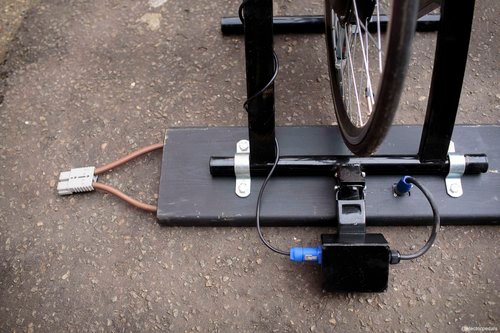
\includegraphics[keepaspectratio=true,scale=0.8]{interacao/11.png}
	 \caption{Gerador com bicicleta acoplada}
	 \small{Fonte: electricpedals.squarespace.com}
	\end{figure}
	
Os distribuidores Bus Board são usados para conectar-se rapidamente acima dos pares de qualquer um dos geradores de energia. Eles também fornecem uma plataforma estável para as pessoas a entrar e sair das bicicletas e garantir que não há nenhum cabo solto.

	\begin{itemize}

	\item Características
	
	O design modular significa facilidade de configuração e arranjo.Pares de alumínio embutidos na base da placa, super base estável para a montagem segura de bicicletas. Perfil \textit{flush} para fácil armazenamento, usa conectores bloqueáveis, extremamente robustos e confiáveis.				
	\end{itemize}	
			
	\begin{itemize}
	\item Vantagens
		Temos como vantagens uma configuração rápida, permitindo um grande número de geradores de fricção de bicicleta e geradores de cubo de bicicleta. Possue uma grande estabilidade, porque eles estão dispostos aos pares, cada pessoa fornece um lastro para a pessoa oposta. Os cabos são bem guardados para que as pessoas não venham tropeçar. Seu armazenamento é facilitado, pela falta de peças elevadas.	
	\end{itemize}		

	\begin{itemize}
	\item Especificações
		Suporte para duas unidades de geração de energia. Com um peso de 14,2 Kg. Um conector de bateria de 175 A ligados através de um cabo de cobre de 35 milímetro$s^{2}$. Com dimensões de L240cm x P21.5cm x H4.5cm
	\end{itemize}	

	\begin{itemize}
	\item Especificação de bicicleta para geração de energia
		O melhor tipo de bicicleta para a geração de energia é uma bicicleta estrada ou híbrido. Seus pneus traseiros lisos irá manter tanto ruído e fricção a um mínimo assegurando, e a melhor de transferência de energia.
	\end{itemize}
	
	\begin{itemize}
		\item Qualidades essenciais (Bicicleta para adulto)
		
		Engrenagens : Pelo menos cinco marchas para permitir o ajuste da geração de energia (sem fixie / bicicletas de velocidade única).
	
	\begin{figure}[H]
	 \centering
	\label{Engrenagem adequada}
	 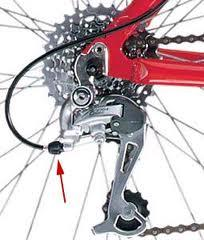
\includegraphics[keepaspectratio=true,scale=0.8]{interacao/12.png}
	 \caption{Engrenagem adequada}
	 \small{Fonte: electricpedals.squarespace.com}
	\end{figure}
	
	\begin{figure}[H]
	 \centering
	\label{Engrenagem inadequada}
	 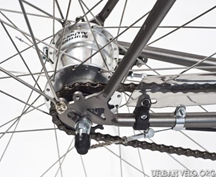
\includegraphics[keepaspectratio=true,scale=0.8]{interacao/13.png}
	 \caption{Engrenagem inadequada}
	 \small{Fonte: electricpedals.squarespace.com}
	\end{figure}		
	
	Pneus: Deve ter um pneu traseiro liso (ou, pelo menos, um padrão de piso consistente) . 
	
	\begin{figure}[H]
	 \centering
	\label{Pneu adequado}
	 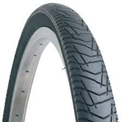
\includegraphics[keepaspectratio=true,scale=0.8]{interacao/14.png}
	 \caption{Pneu adequado}
	 \small{Fonte: electricpedals.squarespace.com}
	\end{figure}
	
	\begin{figure}[H]
	 \centering
	\label{Pneu inadequado}
	 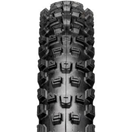
\includegraphics[keepaspectratio=true,scale=0.8]{interacao/15.png}
	 \caption{Pneu inadequado}
	 \small{Fonte: electricpedals.squarespace.com}
	\end{figure}
	
	\end{itemize}
	
	\begin{itemize}
	\item Qualidades opcionais
	
	Pequeno quadro : Para permitir que pessoas de todos os tamanhos possam andar de bicicleta. ( 14 "ou 15" ).

	Assento de liberação rápida : Para permitir o ajuste para ciclistas de diferentes tamanhos.
	
	Passo através do quadro : Para permitir a facilidade de entrar e sair. 
	
	\begin{figure}[H]
	 \centering
	\label{Bicicleta adequada}
	 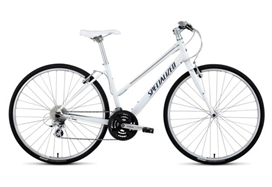
\includegraphics[keepaspectratio=true,scale=0.8]{interacao/16.png}
	 \caption{Bicicleta adequada}
	 \small{Fonte: electricpedals.squarespace.com}
	\end{figure}
		
	\end{itemize}
\end{itemize}

\subsubsection{Aplicativo}

	O avanço da tecnologia, tem tornado as pessoas cada vez mais próximas, independente da distância. Essa aproximação se dá, na maioria das vezes, por meio das redes sociais, sejam elas sites ou aplicativos. Devido a esse fato, pensou-se na ideia da criação de um aplicativo para o Parque Vivencial Urbano do Gama, o qual qualquer pessoa poderá baixá-lo em seu \textit{smartphone}.
	
	A interface inicial do aplicativo possuirá links, como mapa do parque, agenda de eventos, texto descritivo e galeria de fotos do mesmo. Ao clicar no mapa o usuário terá acesso a uma lista de locais, como \textit{playgrounds}, aparelhos para exercícios físicos, quiosques, banheiros, estacionamentos, nascentes e espaço de eventos. Para saber suas respectivas localizações e sobre o parque, basta clicar no local desejado e irá aparecer um outro mapa indicando sua localização e um \textit{link} que levará à descrição. Clicando na agenda será aberta uma lista dos tipos de eventos, dentre eles estão música, teatro e exposições. Para saber as atrações e as datas o usuário deve clicar no evento desejado. Ele também encontrará a descrição do mesmo.

	Além de tudo, as pessoas podem interagir entre si, por exemplo, comentar como está sendo um evento, comentar as fotos e sobre os locais onde elas estão naquele momento. Para isso é preciso fazer um rápido cadastro. Dessa forma, o parque se tornará mais atrativo, estimulando assim, as pessoas a frequentá-lo. 
Abaixo segue as imagens do aplicativo do Parque Ibirapuera, localizado em São Paulo, que serviu como exemplo para a criação do aplicativo para o Parque do Gama.

\begin{figure}[H]
	 \centering
	\label{Pagina inicial do aplicativo}
	 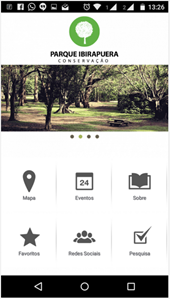
\includegraphics[keepaspectratio=true,scale=0.8]{interacao/17.png}
	 \caption{Pagina inicial.}
\end{figure}
	
\begin{figure}[H]
	 \centering
	\label{Seleção da opção para visualização do mapa}
	 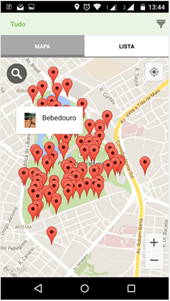
\includegraphics[keepaspectratio=true,scale=0.8]{interacao/18.png}
	 \caption{Seleção da opção para visualização do mapa.}
\end{figure}

\begin{figure}[H]
	 \centering
	\label{Seleção da opção para visualização da lista de locais}
	 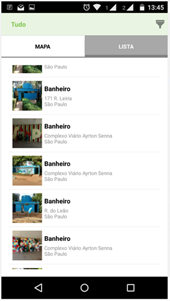
\includegraphics[keepaspectratio=true,scale=0.8]{interacao/19.png}
	 \caption{Seleção da opção para visualização da lista de locais.}
\end{figure}
	
\begin{figure}[H]
	 \centering
	\label{Seleção do local}
	 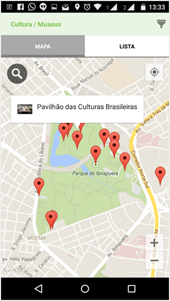
\includegraphics[keepaspectratio=true,scale=0.8]{interacao/20.png}
	 \caption{Seleção do local.}
\end{figure}

\begin{figure}[H]
	 \centering
	\label{Visualização de informações do local}
	 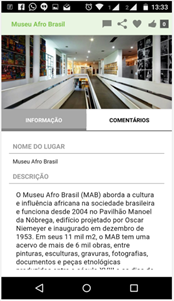
\includegraphics[keepaspectratio=true,scale=0.8]{interacao/21.png}
	 \caption{Visualização de informações do local.}
\end{figure}
\begin{figure}[H]
	 \centering
	\label{Seleção do local}
	 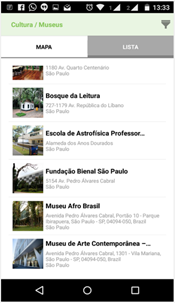
\includegraphics[keepaspectratio=true,scale=0.8]{interacao/22.png}
	 \caption{Seleção do local.}
\end{figure}
\begin{figure}[H]
	 \centering
	\label{Seleção para especificação do evento}
	 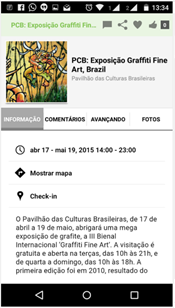
\includegraphics[keepaspectratio=true,scale=0.8]{interacao/23.png}
	 \caption{Seleção para especificação do evento.}
\end{figure}

\subsubsection{Ecoquiosques e postes com tomadas e acesso à \textit{Wi-Fi}}
	
	Atitudes ecológicas cada vez mais tem sido vistas como prioridade e assunto de extrema importância na atualidade em todo o mundo. Essas atitudes podem começar com pequenos gestos, com suas aplicações cada vez mais presentes no cotidiano das pessoas, inclusive em quiosques com aplicações sustentáveis.

	Como o  Parque Urbano do Gama já conta com um quiosque praticamente pronto em alvenaria. Um exemplo útil e prático se vê no desenvolvimento ou reaproveitamento de quiosques com visão sustentável, que apesar de poderem ser feitos em alvenaria possuem equipamentos de captação de luz solar, ou seja, placas fotovoltaicas que armazenam energia e contribuem para a iluminação e aquecimento do local,  tudo isso visando a economia de energia. Sua iluminação pode ser feita com luzes de \textit{LED}, pois além de serem extremamente mais econômicas, têm maior durabilidade. Outro aspecto importante desses quiosques sustentáveis, são os sistemas de coleta e reutilização da água da chuva. Já que abaixo do telhado, que possui um declive, encontra-se um tanque de armazenamento de água da chuva coletada pela cobertura do local.
	
\begin{figure}[H]
	 \centering
	\label{Modelo de quiosque ecólogico}
	 \includegraphics[keepaspectratio=true,scale=0.8]{interacao/24.png}
	 \caption{Modelo de quiosque ecólogico.}
	 \small{Fonte: yankodesign.com/2011/04/08/ecokios/}
\end{figure}

\subsubsection{\textit{Wi-Fi} e Postes com \textit{USB} no parque do Gama}
	
	É notório que a internet e os smartphones vieram pra ficar e a cada dia mais estão  presentes na vida das pessoas. O conceito de disponibilizar rede \textit{Wi-Fi} de internet e postes com conectores \textit{USB} para recarga de bateria de celulares no Parque Urbano do Gama, se deu justamente pra trazer atrativos a mais para a revitalização do mesmo, e consequentemente mais visitantes ao local. A população poderá utilizar a rede pra diversas atividades, com as principais sendo o lazer e os estudos.

	O conceito de \textit{Wi-Fi} livre surgiu através de um modelo já adotado em São Paulo – SP. Na cidade, a rede pertencente a praça Padre Aleixo Monteiro Mafra, conhecida como Praça do Forró, funciona 24 horas e comporta conexão simultânea de até 50 pessoas. Programas semelhantes ao Wi-fi Livre Parque Urbano Gama funcionam em cidades como Barcelona e Berlim. 	

	A velocidade da rede será de 512 Kbps por usuário, já que serão instalados três links de 25 Mpbs, o que permitirá atender até 150 usuários simultâneamente, algo que dependerá de 03 roteadores \textit{Mikrotik/RouterBoard} modelo 1100. Para acessar a internet gratuita no Parque Urbano do Gama com o sistema em operação, o usuário deverá conectar seu smartphone, tablet ou nootbook na rede de \textit{Wi-Fi} do Parque, além de efetuar a autenticação por meio de um navegador de internet.
		
	Por outro lado, para iluminação do ambiente onde ficarão os quiosques ecológicos e onde a \textit{Wi-Fi} será estabelecida, serão implementados postes com técnologia de placas solares de 15 watts, que também possuirão conectores \textit{USB} para que os visitantes possam utilizar mais esse recurso oferecido pelo Parque Urbano do Gama.
	
	Já esta outra idéia surgiu no Brooklyn, mais especificamente no \textit{Fort Green Park}. São postes com suportes para apoio dos celulares por meio de conexão mini \textit{USB}, iphone 4 e 5. As estruturas possuem três placas fotovoltaicas e baterias que armazenam a energia produzida. As baterias são  capazes de absorverem raios UV quando os dias estão nublados e podem ser carregas em até quatro horas nos dias de sol.

\begin{figure}[H]
	 \centering
	\label{Praça do forró em São Paulo}
	 \includegraphics[keepaspectratio=true,scale=0.8]{interacao/25.png}
	 \caption{Praça do Forro em São Paulo.}
	 \small{Fonte:wifilivre.sp.gov.br/}
\end{figure}

\begin{figure}[H]
	 \centering
	\label{Poste com placa fotovoltaíca}
	 \includegraphics[keepaspectratio=true,scale=0.8]{interacao/26.png}
	 \caption{Poste com placa fotovoltaíca no Brooklyn.}
	 \small{Fonte: jblog.jb.com.br/papodeambiente}
\end{figure}

\begin{figure}[H]
	 \centering
	\label{Carregador de celular USB em poste solar no Brooklyn}
	 \includegraphics[keepaspectratio=true,scale=0.8]{interacao/27.png}
	 \caption{Carregador de celular USB em poste solar no Brooklyn.}
	 \small{Fonte: jblog.jb.com.br/papodeambiente}
\end{figure}	

\subsection{Postes Solares}

\subsubsection{Estudo comparativo das tecnologias dos postes}
	O estudo realizado têm como propósito comparar tecnologias existentes no mercado utilizadas na iluminação pública utilizando placas solares, baterias e lampadas \textit{LED}, para auxiliar na revitalização do Parque Urbano e Vivencial do Gama. Com base em tal pesquisa, realizou-se a escolha do poste, visando aspectos econômicos, financeiros e tecnológicos, além de fazer um balanço energético da energia produzida, e consumida pelos postes.

	O levantamento realizado mostrou que existem vários tipos de postes solares atualmente no mercado, os quais possuem  tecnologias diversas com aplicações distintas e em vários ambientes públicos.  Abaixo serão apresentados os estudos desses.

\begin{itemize}
	\item PIE - Produtor Independente de Energia
	
	Foi desenvolvido um poste autossustentável denominado PIE (Produtor Independente de Energia), no Ceará, pelo engenheiro mecânico e dono da \textit{Gram-Eollic} Fernandes Ximenes, o qual utiliza energia solar e eólica e contém baterias para armazenar a produção, obtendo uma autonomia de até sete dias apenas com o armazenado nas mesmas, considerando carga total. Segundo Ximenes, “as baterias do poste híbrido têm autonomia para 70 horas, ou seja, caso falte vento e sol 470 horas, ou sete noites seguidas, as lâmpadas continuarão ligadas.” Cada poste é capaz de abastecer outros três ao mesmo o tempo. O poste é portanto um gerador e é capaz de produzir energia para outros dois postes sem gerador e com seis lâmpadas \textit{LEDs}. 
	
	\begin{figure}[H]
	 \centering
	\label{Produtor independente de energia}
	 \includegraphics[keepaspectratio=true,scale=0.8]{postes/1.png}
	 \caption{PIE - Produtor independente de energia.}
	 \small{Fonte: http://www.conversaafiada.com.br/economia/2010/04/20/energia-eolica-e-solar-o-brasil-que-o-pig-pignora}
	\end{figure}

\end{itemize}

\begin{itemize}
	\item Ecoposte da \textit{Savwatt}
	
	A empresa \textit{Savwatt}, especializada em lâmpadas \textit{LED}, está produzindo, também, um poste auto sustentável alimentado a energia solar e eólica. O poste é constituido de materiais bem resistentes e é fácil de ser instalado. O produto já esta sendo comercializado nos EUA.
	
	\begin{figure}[H]
	 \centering
	\label{Ecoposte da savatt}
	 \includegraphics[keepaspectratio=true,scale=0.8]{postes/2.png}
	 \caption{Ecoposte da savatt.}
	 \small{Fonte: https://www.flickr.com/photos/56798891@N05/5246662531/in/set-72157625564235580}
	\end{figure}

\end{itemize}
	
\begin{itemize}
	 \item Poste \textit{Sunlab} Linha Malibú
	
	A seguir são apresentados 2 tipos de postes produzidos pela \textit{Sunlab}, empresa com atuação global que possui sede no Brasil e fabrica postes solares.
	
	O primeiro poste analisado, produzido pela \textit{Sunlab}, corresponde à sua linha de produção Malibú. Esta linha corresponde a um equipamento de última geração, que harmoniza o avanço tecnológico com a consciência da utilização de energias alternativas e apresenta dois modelos no mercado.

	Os modelos produzidos são o LPZ e  LY. O Malibú LPZ é um modelo fácil de instalar que não requer qualquer instalação elétrica, bastando fixá-lo ao solo em local exposto ao Sol. Ele é leve e compacto podendo ser transportado e desmontado com facilidade. Além disso, gera sua própria energia através do painel solar, utilizando bateria para armazenamento da mesma, especial para descarga profunda (acumula a energia necessária para o funcionamento a noite inteira). Ele ainda possui durabilidade de até 50.000 horas (mais de 10 anos, trabalhando  12 horas toda noite), e seus \textit{LEDs} não possuem radiação que possa danificar materiais sensíveis ou animais.  Ele também possui sensor lógico, que liga a noite e desliga automaticamente de dia, sem qualquer intervenção humana ou gasto de energia.

	O Malibú LY possui praticamente as mesmas características, diferindo apenas em alguns aspectos técnicos, tais como a quantidade  de luminárias por poste, a quantidade de placas, a capacidade de armazenamento das baterias, e a área de cobertura da iluminação. As vantagens para ambos os sistemas de iluminação são: 

	\begin{itemize}
		\item Custo "zero" de energia elétrica;
		\item Instalação simples e barata;
		\item Alta durabilidade e confiabilidade;
		\item Baixo custo de manutenção;
		\item Não necessita a troca de lâmpadas;
		\item A bateria tem uma vida média de 2 anos tendo sua troca e descarte através da Sunlab Power.
	\end{itemize}
	
	\begin{enumerate}
		\item Modelo LZP
		
	O modelo LZP é uma linha tradicional, desenvolvido para a iluminação externa com o uso da energia solar. É um equipamento de tecnologia sofisticada para iluminação, fornecido completo e pronto para o funcionamento. \cite{SUNLAB} 

	Cada unidade é auto suficiente, possui seu próprio gerador de eletricidade,  a bateria para acumular a energia e um circuito eletrônico micro controlado para sua recarga e automação. O esquemático da figura (a) mostra um modelo desse tipo e a figura (b) mostra a cobertura em área pela irradiação da luz.
		
	\end{enumerate}
	
	\begin{figure}[H]
	 \centering
	\label{Modelo de poste A}
	 \includegraphics[keepaspectratio=true,scale=0.8]{postes/3.png}
	 \caption{Modelo de poste A.}
	 \small{Fonte: sunlab.com.br}
	\end{figure}
	
	\begin{figure}[H]
	 \centering
	\label{Modelo de poste B}
	 \includegraphics[keepaspectratio=true,scale=0.8]{postes/4.png}
	 \caption{Modelo de poste B}
	 \small{Fonte: sunlab.com.br}
	\end{figure}
		
	O painel solar gera eletricidade uma vez exposto à luz do Sol e o controlador armazena na bateria, energia suficiente para uma autonomia de até 24 horas, variando a capacidade de acordo com o modelo do LZP, como mostrado na tabela a seguir.
	
	As fontes de luz são potentes emissores de estado sólido:  de acordo com a tabela 1, os modelos do tipo LZP possuem características muito distintas e importantes, tais como  materiais de alta durabilidade, recicláveis, tendo um baixo impacto ao meio ambiente e mínima manutenção e sem custo de energia ou infraestrutura de instalação.  	Possui ainda os power \textit{LEDs}, que são muito mais econômicos se comparados às lâmpadas convencionais e de altíssima duração.
\end{itemize}

	\begin{figure}[H]
	 \centering
	\label{Caractéristicas do poste}
	 \includegraphics[keepaspectratio=true,scale=0.8]{postes/tabelaLZP.png}
	 \caption{Caractéristicas do poste.}
	 \small{Fonte: sunlab.com.br}
	\end{figure}


\begin{table}[H]
\center
\caption{Características do poste Malibú modelo LZP}
\small{sunlab.com.br}
\begin{tabular}{lllll}
 &  &  &  &  \\ \hline
\multicolumn{1}{|l|}{\textbf{Modelo}} & \multicolumn{1}{l|}{\textbf{LZP 102}} & \multicolumn{1}{l|}{\textbf{LZP 104}} & \multicolumn{1}{l|}{\textbf{LZP 204}} & \multicolumn{1}{l|}{\textbf{LZP 208}} \\ \hline
\multicolumn{1}{|l|}{\textit{Código do produto}} & \multicolumn{1}{l|}{96.500} & \multicolumn{1}{l|}{96.501} & \multicolumn{1}{l|}{96.503} & \multicolumn{1}{l|}{96.504} \\ \hline
\multicolumn{1}{|l|}{\textit{Qt.de refletores (pétala)}} & \multicolumn{1}{l|}{1} & \multicolumn{1}{l|}{1} & \multicolumn{1}{l|}{2} & \multicolumn{1}{l|}{2} \\ \hline
\multicolumn{1}{|l|}{\textit{Qt. de emissores de luz}} & \multicolumn{1}{l|}{4} & \multicolumn{1}{l|}{8} & \multicolumn{1}{l|}{2 x 4} & \multicolumn{1}{l|}{2 x 8} \\ \hline
\multicolumn{1}{|l|}{\textit{Fluxo luminoso (lm)}} & \multicolumn{1}{l|}{400} & \multicolumn{1}{l|}{800} & \multicolumn{1}{l|}{800} & \multicolumn{1}{l|}{1.600} \\ \hline
\multicolumn{1}{|l|}{\textit{\begin{tabular}[c]{@{}l@{}}Iluminância ao nível \\ do solo (lux)*\end{tabular}}} & \multicolumn{1}{l|}{15} & \multicolumn{1}{l|}{20} & \multicolumn{1}{l|}{18} & \multicolumn{1}{l|}{38} \\ \hline
\multicolumn{1}{|l|}{\textit{Peso (Kg)}} & \multicolumn{1}{l|}{13} & \multicolumn{1}{l|}{15} & \multicolumn{1}{l|}{17} & \multicolumn{1}{l|}{24} \\ \hline
\multicolumn{1}{|l|}{\textit{Tensão de trabalho (Vdc)}} & \multicolumn{1}{l|}{12} & \multicolumn{1}{l|}{12} & \multicolumn{1}{l|}{12} & \multicolumn{1}{l|}{12} \\ \hline
\multicolumn{1}{|l|}{\textit{Aplicação}} & \multicolumn{4}{l|}{Iluminação de jardins, parques, passeios, etc..} \\ \hline
\multicolumn{1}{|l|}{\textit{Alimentação}} & \multicolumn{4}{l|}{Através do painel solar fotovoltaico.} \\ \hline
\multicolumn{1}{|l|}{\textit{Bateria}} & \multicolumn{4}{l|}{Eletrolítica de ciclo profundo.} \\ \hline
\multicolumn{1}{|l|}{\textit{Acionamento}} & \multicolumn{4}{l|}{Automático.} \\ \hline
\multicolumn{1}{|l|}{\textit{Autonomia c/ 50\% de insolação}} & \multicolumn{4}{l|}{\textgreater 24 horas} \\ \hline
\multicolumn{1}{|l|}{\textit{Cor da luz}} & \multicolumn{4}{l|}{Branca (5.000 - 5.500K).} \\ \hline
\multicolumn{1}{|l|}{\textit{Corpo}} & \multicolumn{4}{l|}{\begin{tabular}[c]{@{}l@{}}Em aço com tratamento anticorrosivo \\ e pintura eletrostática.\end{tabular}} \\ \hline
\multicolumn{1}{|l|}{\textit{Fixação}} & \multicolumn{4}{l|}{\begin{tabular}[c]{@{}l@{}}Ao solo através de fixadores / buchas\\  e parafusos (não fornecidos).\end{tabular}} \\ \hline
\multicolumn{1}{|l|}{\textit{Acompanha}} & \multicolumn{4}{l|}{\begin{tabular}[c]{@{}l@{}}Módulo solar, controlador, emissores de luz, \\ bateria e manual de montagem.\end{tabular}} \\ \hline
\multicolumn{1}{|l|}{\textit{Altura}} & \multicolumn{4}{l|}{2,5 metros.} \\ \hline
\multicolumn{1}{|l|}{\textit{Cobertura média iluminada}} & \multicolumn{4}{l|}{6 metros de raio ou 37 m2.} \\ \hline
\multicolumn{1}{|l|}{\textit{Vida útil estimada}} & \multicolumn{4}{l|}{50.000 horas} \\ \hline
\multicolumn{1}{|l|}{\textit{Norma NBR 6164}} & \multicolumn{4}{l|}{IP-44} \\ \hline
\multicolumn{1}{|l|}{\textit{Garantia}} & \multicolumn{4}{l|}{1 (Hum) ano.} \\ \hline
\multicolumn{1}{|l|}{\textit{*Observações:}} & \multicolumn{4}{l|}{\begin{tabular}[c]{@{}l@{}}Media do 1º quadrante de 1 $m^{2}$. . \\ Temperatura= 25º C, Tolerância +/- 15\%\end{tabular}} \\ \hline
\end{tabular}
\end{table}

\begin{enumerate}
	\item Modelo LY
	
	  O modelo  LY  da linha Malibú, foi desenvolvido para atender a iluminação externa em jardins, pátios, parques, estacionamentos, entre outras áreas aplicáveis.
	  
	Seu \textit{design} moderno o identifica com a arquitetura contemporânea, além de ser um equipamento de tecnologia sofisticada para iluminação, fornecido completo e pronto para ser instalado e colocado em funcionamento. Sua fonte de luz é \textit{Power LED} - emissores de luz de estado sólido de alta potência e baixo consumo. Os \textit{LEDs} não aquecem como as lâmpadas e sua vida útil é maior que 50.000 horas ( mais de 11 anos, se aceso 12 horas por noite). \cite{SUNLAB}
    
    O sistema é autônomo, auto sustentável, ecológico e durável. O funcionamento será constante, acendendo automaticamente à noite e apagando durante o dia, sem qualquer intervenção humana ou gasto de energia.
    
    Possui boa durabilidade, baixíssimo impacto ecológico e mínima manutenção, sem custo de energia e infraestrutura de instalação, permitindo que haja o retorno de investimento em curto espaço de tempo, características do modelo LY  que podem ser observadas na tabela abaixo.

	\begin{figure}[H]
	 \centering
	\label{Caractéristicas do poste LY}
	 \includegraphics[keepaspectratio=true,scale=0.8]{postes/tabelaLY.png}
	 \caption{Caractéristicas do poste LY.}
	 \small{Fonte: sunlab.com.br}
	\end{figure}


\begin{table}[H]
\center
\caption{Características do poste Malibú modelo LY}
\small{Fonte: sunlab.com.br}
\begin{tabular}{llllll}
 &  &  &  &  &  \\ \hline
\multicolumn{1}{|l|}{\textbf{Modelo}} & \multicolumn{1}{l|}{\textbf{LY - 104}} & \multicolumn{1}{l|}{\textbf{LY - 108}} & \multicolumn{1}{l|}{\textbf{LY - 204}} & \multicolumn{1}{l|}{\textbf{LY - 208}} & \multicolumn{1}{l|}{\textbf{LY - 216}} \\ \hline
\multicolumn{1}{|l|}{\textbf{Código do produto}} & \multicolumn{1}{l|}{\textbf{96.502}} & \multicolumn{1}{l|}{\textbf{96.505}} & \multicolumn{1}{l|}{\textbf{96.506}} & \multicolumn{1}{l|}{\textbf{96.507}} & \multicolumn{1}{l|}{\textbf{96.511}} \\ \hline
\multicolumn{1}{|l|}{\textit{Qt.de refletores (pétala)}} & \multicolumn{1}{l|}{1} & \multicolumn{1}{l|}{1} & \multicolumn{1}{l|}{2} & \multicolumn{1}{l|}{2} & \multicolumn{1}{l|}{2} \\ \hline
\multicolumn{1}{|l|}{\textit{Qt. de emissores de luz}} & \multicolumn{1}{l|}{4} & \multicolumn{1}{l|}{8} & \multicolumn{1}{l|}{2 x 4} & \multicolumn{1}{l|}{2 x 8} & \multicolumn{1}{l|}{2 x 14} \\ \hline
\multicolumn{1}{|l|}{\textit{Fluxo luminoso (lm)}} & \multicolumn{1}{l|}{400} & \multicolumn{1}{l|}{800} & \multicolumn{1}{l|}{800} & \multicolumn{1}{l|}{1.600} & \multicolumn{1}{l|}{2.800} \\ \hline
\multicolumn{1}{|l|}{\textit{\begin{tabular}[c]{@{}l@{}}Iluminância ao nível \\ do solo (lux)*\end{tabular}}} & \multicolumn{1}{l|}{15} & \multicolumn{1}{l|}{20} & \multicolumn{1}{l|}{18} & \multicolumn{1}{l|}{38} & \multicolumn{1}{l|}{49} \\ \hline
\multicolumn{1}{|l|}{\textit{Peso (Kg)}} & \multicolumn{1}{l|}{13} & \multicolumn{1}{l|}{15} & \multicolumn{1}{l|}{17} & \multicolumn{1}{l|}{24} & \multicolumn{1}{l|}{26} \\ \hline
\multicolumn{1}{|l|}{\textit{Aplicação}} & \multicolumn{5}{l|}{Iluminação de jardins, parques, passeios, etc..} \\ \hline
\multicolumn{1}{|l|}{\textit{Alimentação}} & \multicolumn{5}{l|}{Painel solar fotovoltaico 12 / 24 Vdc.} \\ \hline
\multicolumn{1}{|l|}{\textit{Bateria}} & \multicolumn{5}{l|}{Eletrolítica / Gel, de ciclo profundo.} \\ \hline
\multicolumn{1}{|l|}{\textit{Acionamento}} & \multicolumn{5}{l|}{Automático.} \\ \hline
\multicolumn{1}{|l|}{\textit{Autonomia c/100\% insolação}} & \multicolumn{5}{l|}{\textgreater 24 horas} \\ \hline
\multicolumn{1}{|l|}{\textit{Cor da luz}} & \multicolumn{5}{l|}{\begin{tabular}[c]{@{}l@{}}Branca (5000 - 5500K) ou outras \\ cores sob encomenda.\end{tabular}} \\ \hline
\multicolumn{1}{|l|}{\textit{Corpo}} & \multicolumn{5}{l|}{\begin{tabular}[c]{@{}l@{}}Em aço com tratamento anticorrosivo \\ e pintura eletrostática.\end{tabular}} \\ \hline
\multicolumn{1}{|l|}{\textit{Lente}} & \multicolumn{5}{l|}{Em vidro branco leitoso.} \\ \hline
\multicolumn{1}{|l|}{\textit{Fixação}} & \multicolumn{5}{l|}{\begin{tabular}[c]{@{}l@{}}Ao solo através de fixadores - buchas\\  e parafusos (não fornecidos).\end{tabular}} \\ \hline
\multicolumn{1}{|l|}{\textit{Acompanha}} & \multicolumn{5}{l|}{\begin{tabular}[c]{@{}l@{}}Módulo solar, controlador eletrônico, \\ emissores de luz, bateria e manual de montagem.\end{tabular}} \\ \hline
\multicolumn{1}{|l|}{\textit{Altura padrão}} & \multicolumn{5}{l|}{2,5 metros.} \\ \hline
\multicolumn{1}{|l|}{\textit{Cobertura média iluminada}} & \multicolumn{5}{l|}{36 m2.} \\ \hline
\multicolumn{1}{|l|}{\textit{Vida útil estimada}} & \multicolumn{5}{l|}{50.000 horas} \\ \hline
\multicolumn{1}{|l|}{\textit{Norma NBR 6164}} & \multicolumn{5}{l|}{IP-44} \\ \hline
\multicolumn{1}{|l|}{\textit{Garantia}} & \multicolumn{5}{l|}{1 (Hum) ano.} \\ \hline
\multicolumn{1}{|l|}{\textit{*Observações:}} & \multicolumn{5}{l|}{\begin{tabular}[c]{@{}l@{}}Media do 1º quadrante em 1 $m^{2}$, tensão = 12,5V,\\  temperatura= 25º C, Tolerância +/- 15\%\end{tabular}} \\ \hline
\end{tabular}
\end{table}

\end{enumerate}

\begin{itemize}
	\item Poste \textit{Sunlab} linha PTS
	
	O segundo poste analisado, também  produzido pela \textit{Sunlab}, corresponde à linha PTS, e ao seu kit fornecido para iluminação pública. Ela foi elaborada para quem deseja instalar postes de iluminação alimentados a energia SOLAR com luminária a \textit{LED} de alta potência.
	
	O sistema é composto por:
	\begin{itemize}
	\item Luminária a LED ILC (várias potencias);
	\item Braço de fixação da luminária;
	\item Painel solar;
	\item Suporte articulado do painel solar;
 	\item Gabinete de baterias; 
 	\item Baterias de Ciclo Profundo para trabalhar com energia solar;
	\item Controlador inteligente, para carga e descarga das baterias com função fotossensora;
 	\item Dispositivo de proteção contra falhas;
	\item Conexões através de bornes para fios até 6 m$m^{2}$;
	\item Cabos elétricos e conectores para todo o sistema;
	\end{itemize}
	
	O poste é fornecido opcionalmente, flangeado ou engastado, desmontável para fácil transporte. São, dimensionalmente, calculados para dar a segurança quanto ao peso e ventos acima de 150 km/h. São galvanizados a fogo para aumentar sua resistência mecânica.
	
	Características:
	
	\begin{itemize}
	\item Dimensionado para manter iluminado a noite inteira e com reserva para dias de baixa insolação.
	\item Suporte articulado de sustentação do painel solar, com regulagem angular e de direção. 
 	\item Opcionalmente fabricados com sistemas híbridos, ligados ao solar e à uma segunda fonte de energia, que pode ser acionada como back up. 
	\item Braço da luminária longo, médio ou curto, opções para sua aplicação.
Gabinete IP 65, apropriado para conter baterias, controlador de carga e demais partes elétricas.
	\end{itemize}

    Vantagens, de acodo com o manual do fabricante:
    \begin{itemize}
    \item Economia: Sistemas a energia solar não tem conta de energia. Invista no equipamento e usufrua da iluminação por anos.
	\item Economia na instalação: Eliminam a fiação como dos postes tradicionais, quadros, disjuntores, reatores, etc.
	\item Resistência: Alta durabilidade dos componentes. Não suscetível a quebra por vibrações provocadas na passagem de veículos ou a variações repentinas de clima e temperatura. Não possui peças móveis sujeitas a desgaste. As luminárias LED tem vida útil de 50.000 horas de uso e painéis solares tem mais de 30 anos.
	\item Segurança: A luminária opera com módulos LED independentes. Na eventual falha de um, permanece acesa mesmo que parcialmente, reduzindo a possibilidade de falta de luz e consequentes acidentes.
	\item Segurança II: A aplicação de temperatura de cor mais elevada, permite reduzir o  fluxo de iluminação, sem perda da acuidade visual, resultando em melhor distinção do espaço, sombras e cores. Maior nitidez das cores e melhor visualização de objetos em movimento, sem ofuscamento.
 	\item Versatilidade: Iluminação uniforme, sem radiações que possam prejudicar ou cansar a visão. Permite ser instalado em postes já existentes, com poucas adaptações.
	\item Ecologicamente correto: Não contém substâncias nocivas à saúde humana e à natureza. As partes são remanufaturáveis e não precisam ser descartadas. Durabilidade muito acima dos componentes tradicionais.
	\item Manutenção Corretiva: Depende da escolha da tecnologia do acumulador.Trocas preventivas podem ser necessárias entre 3 a 8 anos, conforme a escolha.  Não há trocas de lâmpadas ou reator como na iluminação convencional.
    \end{itemize}

\end{itemize}

\subsubsection{Poste a ser aplicado}
	Comparando as tecnologias e os vários modelos, pode-se perceber discrepâncias  entre alguns fatores muito importantes para as funções que irão desempenhar no Parque, tais como a altura do poste e a irradiação e disseminação da luz proporcionadas pelos mesmos. 
	
	Optou-se pela utilização dos postes da empresa \textit{Sunlab}, em específico o kit de iluminação pública da linha PTS. A escolha é justificada pelo maior acesso às informaçoes técnicas que a empresa disponibiliza, quando comparada às outras empresas e tecnologias pesquisadas.
	
	Os modelos da linha Malibú tem  no máximo 2,5 m de altura e a iluminação é dissipada num raio de 36,0 $m^{2}$ de de distância do poste. O painel solar gera eletricidade, uma vez exposto à  luz do Sol e o controlador gerencia e armazena na bateria que acumula o suficiente para manter a iluminação durante toda a noite e ainda uma reserva para dias nublados. Enquanto os modelos da linha PTS possuem uma variação de 5 a 12 metros de altura e um raio de iluminação que varia de 452$m^{2}$ para o modelo PTS-320/330 (que chega até 8 metros de altura), a  934,8$m^{2}$ para o modelo PTS-530 (que chega a 12 metros de altura). Além disso, os mesmos podem possuir autonomia de até 60 horas, dependendo do modelo e da irradiação solar, na tabela abaixo estão relacionadas as características de todos os sistemas em análise.

\begin{table}[H]
\caption{Comparações técnicas das tecnologias dos postes}
\begin{tabular}{llll}
\hline
\multicolumn{1}{|l|}{\textbf{Modelo}} & \multicolumn{1}{l|}{\textbf{Altura(m)}} & \multicolumn{1}{l|}{\textbf{Área de iluminação($m^{2}$)}} & \multicolumn{1}{l|}{\textbf{Autonomia(horas)}} \\ \hline
\multicolumn{1}{|l|}{\textit{Malibú LZP/ LY}} & \multicolumn{1}{l|}{2,5/2,5} & \multicolumn{1}{l|}{36/37} & \multicolumn{1}{l|}{24h/24h} \\ \hline
\multicolumn{1}{|l|}{\textit{PTS}} & \multicolumn{1}{l|}{De 6 até 12} & \multicolumn{1}{l|}{De 452 até 934,8} & \multicolumn{1}{l|}{60h} \\ \hline
\end{tabular}
\end{table}

	Dessa forma, optou-se pelo poste da empresa \textit{Sunlab}, com o modelo PTS, pois ele atende às necessidades de iluminação de grandes áreas, sem a necessidade de infraestrutura eletrica para a instalação, proporcionando maior segurança ao Parque. Ademais, tal empresa atende às normas mais rigorosas proporcionando qualidade, segurança, economia, eficiência e durabilidade.
 
	Dois modelos foram escolhidos, um para as áreas de convivência, e outro para as áreas de pistas de corrida. Para as áreas de vivências o modelo escolhido foi o PTS-410 ele tem 8 metros de altura e possui duas luminárias, para diminuir a intensidade luminosa e proporcionar maior conforto aos usuários, pois postes muitos pequenos apresentam grande intensidade luminosa. Para as áreas de pistas de corrida o modelo escolhido foi o PTS-315, pois possui uma única luminária e proporciona maior conforto aos usuários durante a noite, e apresenta boa eficiência energética por parte da placa.

\begin{itemize}
	\item Sistema PTS
	A linha PTS, foi desenvolvida pela \textit{SunLab Power} para introduzir no mercado o conceito de iluminação solar e a emissão de luz: através de LEDs de alta potência. 
	
	O sistema PTS é composto pela luminária(s) a LED, braço de sustentação, painel(is) solar(es) com seu suporte articulado para regulagem e fixação no topo do poste e gabinete contendo o controle eletrônico e bateria(s), conforme mostra a figura 4.
	
	\begin{figure}[H]
	 \centering
	\label{Principais componentes do poste}
	 \includegraphics[keepaspectratio=true,scale=0.8]{postes/5.png}
	 \caption{Principais componentes do poste.}
	 \small{Fonte: sunlab.com.br}
	\end{figure}
	
	Para cada aplicação há capacidades diferentes, potência de iluminação e cobertura, para atender à s necessidades em ruas, parques, estacionamentos, praças, pátios, avenidas. A linha PTS foi desenvolvida em conformidade a norma NBR 5101/92. 
	
	Cada PTS possui funcionamento automático e é auto-suficiente. Opera sem a intervenção humana. O sensor de luminosidade que comanda o acender e apagar é o próprio painel solar. O PTS liga ao escurecer e apaga quando amanhece. Para o acionamento manual, pode ser solicitado como opcional. 
	
	Não necessita de conexão à  rede elétrica.  Devido à  ausência de U.V. (ultravioleta) a atração sobre insetos é reduzida. Isso evita a necessidade de limpeza constante. Pela mesma razão, não há o amarelamento e envelhecimento de partes, provocados pela luz da luminária.  Na falha de um módulo, os outros permanecem funcionando, reduzindo a possibilidade de acidentes.  A luz imediata, ou seja, os emissores de luz a LED não precisam de tempo para aquecimento ou de espera para iniciar a luz, e  o acender e apagar não danifica os emissores LED.
	
	Não oferece qualquer perigo elétrico a pessoas. Trabalha com tensões baixas: em 12 ou 24 Volts. Atende como iluminação de emergência.  Baixa temperatura de trabalho e não é suscetível a quebra por vibrações provocadas na passagem de veículos,e não ocorre trincas como ocorre com as lâmpadas. 	
\end{itemize}

\subsubsection{Composição do Sistema (Kit para iluminação pública)}

	O sistema é  constituído conforme as especificações do fabricante, bem como as características de cada material utilizado. Os dados abaixo foram obtidos do manual de instalação do poste.
	
	As partes que compõem o sistema são:

\begin{enumerate}
	\item Estrutura – Poste; 
	\item Luminária a LED; 
	\item Braço para instalação da luminária; 
	\item Suporte articulado e Painel solar; 
	\item Caixa de controle - contém o controlador e bateria(s).
\end{enumerate}

	Um esquemático do Poste é mostrado na figura abaixo:
	
\begin{figure}[H]
	 \centering
	\label{Esquemático do poste com duas iluminárias}
	 \includegraphics[keepaspectratio=true,scale=0.8]{postes/6.png}
	 \caption{Esquemático do poste com duas iluminárias.}
	 \small{Fonte: sunlab.com.br}
\end{figure}	
	
\begin{enumerate}
	\item Estrutura:
		
	O fornecimento do poste é opcional, no entanto foi determinado para esse projeto o conjunto completo, já que se trata de um parque, cabendo o planejamento das tecnologias aplicadas. Deve ter uma estrutura suficientemente forte para suportar os equipamentos (painéis, braços, luminária) e à  força de arrasto dos ventos.
	
	Projeto o conjunto completo, já que se trata de um parque, cabendo o planejamento das tecnologias aplicadas. Deve ter uma estrutura suficientemente forte para suportar os equipamentos (painéis, braços, luminária) e à  força de arrasto dos ventos. 
	
	Sua base pode ser flangeada ou engastada. A instalação deve ser feita conforme orientação do fabricante e com a utilização de pessoal especializado. Devido ao solo presente no local não poder sofrer muitas alterações, restricões essas devido a Lei N° 12.651/12 do Código Florestal, optou-se pelo poste de estrutura engastada, por não haver a necessidade de colocarmos concreto para a fixação do poste. As figura 32 mostra um esquemático da estrutura do modelo PTS-315, e a figura 33 do modelo PTS-410.

		De acordo com a imagens a iluminação da luminária se expande em cerca de 120°, e a altura do poste para tais modelos chega até 8 metros. Pode-se verificar ainda que  para o modelo PTS-410 a área de iluminação é duplicada pois o mesmo possui duas luminárias, cada luminária ilumina uma área  de 572 $m^{2}$ aproximadamente.


	\item Luminária a LED:
	
	A Luminária ILC possui lente difusora em PPA transparente, uma resina sintética termoplástica da família poliamida (\textit{nylon}) que é usada para substituir metais em aplicações de alta temperatura, resistente à  ação de UV e a intempéries. Além disso, este material é a prova de trincas por vibrações advindas de carros e ou pedestres que frequentem os locais em que os postes estejam instalados. O travamento da lente é feito por fecho rápido de pressão e permite o fácil acesso interno à  mesma. A instalação no braço (3) deve ser através da luva, com o aperto aos dois parafusos do dispositivo de travamento. É permitida a instalação em braços desde 33,7 mm até 61 mm. 
	O circuito de alimentação funciona em PWM, \textit{Pulse Width Modulation} ou Modulação de Largura de Pulso, que funciona como um regulador de potência para o circuito, com proteção contra sobre e sub-tensão, curto-circuito e controle de temperatura, através de duas até quatro setores de alimentação isolados. Cada circuito possui um fusível de proteção, como a figura 8. Por não emitir raios no espectro não visível ultra violeta, a atração de insetos é nula, o que ainda contribui para reduzir a necessidade de limpezas frequentes, reduzindo mais ainda os custos deste modelo de luminária. Na tabela a seguir é possível ver suas principais características, podendo verificar que, a diferença de potência de trabalho da mesma é de 12 a 24 volts, reduzindo assim os riscos de choques elétricos e o desgaste dos componentes eletrônicos, além de tornar o circuito mais simples e leve, necessitando de menos componentes.


\begin{table}[H]
\center
\caption{Características da luminária ILC. Fonte: sunlab.com.br}
\begin{tabular}{|l|l|}
\hline
Luminária ILC                    & linha 315 \\ \hline
Equivalente a (Lâmpada Descarga) & 120W      \\ \hline
Corrente (Ampèrs)                & 3,5       \\ \hline
Grau de Proteção                 & IP-65     \\ \hline
Consumo Máximo (Watts)           & 48        \\ \hline
Tensão de alimentação (VAC)      & 12VDC     \\ \hline
\end{tabular}
\end{table}

\begin{figure}[H]
	 \centering
	\label{Luminária}
	 \includegraphics[keepaspectratio=true,scale=0.8]{postes/9.png}
	 \caption{Luminária.}
	 \small{Fonte: sunlab.com.br}
\end{figure}

	\item Braço para instalação da luminária:
	
	É o segmento onde se instala a luminária. Há vários tipos utilizados (curto/ médio/ longo) e permite desde uma até quatro luminárias. O braço padrão tem 2,5 metros de comprimento e inclinação de 5º graus. Os postes que serão utilizados apresentam  apenas uma luminária para o sistema PTS-315, e duas para o sistema PTS-410.
	
	\item O suporte do(s) painel(is) solar(es):
	
	\'E articulado, metálico, com encaixe para postes cilíndricos de diâmetros desde 2,5”até 6”. Possui regulagem para os painéis tanto na inclinação como na rotação. os diâmetros considerados são de 3” para o modelo PTS-315 e de, 4” para o PTS-410, observe o modelo genérico nas figuras 9 e 10.
	
\begin{figure}[H]
	 \centering
	\label{Vista lateral do suporte}
	 \includegraphics[keepaspectratio=true,scale=0.8]{postes/10.png}
	 \caption{Vista lateral do suporte.}
	 \small{Fonte: sunlab.com.br}
\end{figure}

\begin{figure}[H]
	 \centering
	\label{Vista superior do suporte}
	 \includegraphics[keepaspectratio=true,scale=0.8]{postes/11.png}
	 \caption{Vista superior do suporte.}
	 \small{Fonte: sunlab.com.br}
\end{figure}

	Esse suporte é usado para fixar a placa solar e movimentá-la de acordo com a angulação exigida pela placa no local.

	\item Painel Solar:
	
	De acordo com o fabricante o modelo PTS-315 possui apenas um painel solar, e o modelo PTS-410 2 painéis. Cada região brasileira exige uma angulação diferente para uma produção otimizada de energia pela placa de acordo com a figura 11 abaixo.

\begin{figure}[H]
	 \centering
	\label{Inclinação da placa}
	 \includegraphics[keepaspectratio=true,scale=0.8]{postes/12.png}
	 \caption{Inclinação da placa.}
	 \small{Fonte: sunlab.com.br}
\end{figure}

	\item Gabinete de controle:
	
	Contém a(s) bateria(s) com o circuito controlador de carga e descarga e demais controles de funcionamento de segurança do sistema. O gabinete padrão fornecido é em aço, com pintura epóxi, para fixação no poste, e opcionalmente, há gabinetes em aço inox, fibra, para instalação no solo ou outros materiais específicos. O kit de iluminação pública utilizado corresponde ao gabinete padrão. 
	
	\item Baterias:
	
	No kit padrão é fornecido com baterias eletrolíticas, valvuladas e de ciclo profundo. Seladas e sem necessidade de manutenção. A estimativa de troca é após 4 anos. Outra opção são as baterias \textit{Spiral-Cell}, com o dobro de vida útil. 
De acordo com o fabricante a escolha das bateria deve seguir as seguintes instruções:
Com o total da corrente produzida pelo(s) painé(is), multiplique pelas horas diária de insolação e utilize um fator de segurança:
 
	Os painéis, produzem 50Ah em 12 Volts ou 25Ah em 24V.
Operando por 6 horas de insolação temos:

\begin{center}
	50 Ah x 6 horas = 300 Ampérs dia.
\end{center}
  
	Se a sua escolha for por uma bateria de 100 Ah, e esse acumulador, na prática fosse 100\% utilizável, necessita-se apenas de 3 baterias:

\begin{center}
 300 A/dia Dividido por 100 Ah = 3 Unidades
\end{center}  
 
	Como esse acumulador "ideal" não existe até o momento, temos que optar por uma das melhores tecnologias existentes:
Se sua escolha for por uma bateria  "estacionária" multiplique a necessidade por 2 e arredonde.
Se sua escolha for por uma bateria SpiralCell, multiplique por 1,5 e arredonde.

	Apesar  do custo elevado da bateria spiracell, a mesma será aplicada ao projeto, pois apresenta maior vida útil e maior  capacidade de armazenamento em comparação com a bateria de ciclo profundo. Mostrando-se eficiente e capazes de suprir a demanda armazenando a produção energética das placas solares dos postes.

	Principais vantagens das baterias \textit{Spiralcell}:
	
	\begin{itemize}
	\item Maior resistência e vida útil: suporta 4 vezes mais que qualquer outra bateria convencional.
	\item Placas em espiral com absorventes: retém o eletrólito eliminando vazamentos e resistindo 15 vezes mais a vibrações.
	\item 100\% livre de vazamentos: Podem funcionar inclinadas e podem ser rotadas até 180°.
	\item Recarga até 3 vezes mais rápida.	
	\item Menor peso. 
	\item Alta confiabilidade.
	\item Alta densidade de energia.
	\item Livres de manutenção.
	\item Permitem descarga profunda.
	\end{itemize}

A seguir é apresentado no figura abaixo, um comparativo do rendimento da bateria \textit{Spiralcell} com as baterias convencionais, comprovando sua maior vida útil.

\begin{figure}[H]
	 \centering
	\label{Comparação da bateria spiralcell com as convencionais}
	 \includegraphics[keepaspectratio=true,scale=0.8]{postes/13.png}
	 \caption{Comparação da bateria spiralcell com as convencionais.}
	 \small{Fonte: sunlab.com.br}
\end{figure}

	A bateria \textit{Spiralcell} que melhor se aplica ao parque é a que possui uma maior capacidade de armazenamento, e menor peso, logo de acordo com as baterias fornecidas pelo fabricante a melhor a ser ultilizada é a bateria, cujo código é 93528, e o modelo é  “D31A”. Ela possui uma tenção de 12V, e capacidade de armazenamento de 75Ah, dimensão de 325,5 mm(milímetro), e peso de 27,13kg.


	\item Controlador ZIP:
	
	Totalmente eletrônico e microprocessado, é programado para as operações de liga/desliga da iluminação, controle de carga e descarga da(s) bateria(s), supervisão da quantidade de energia de consumo e proteção dos equipamentos do sistema. Desliga a luminária antes que a bateria se descarregue totalmente e libera o consumo após a recarga, automaticamente, a tabela 6 abaixo mostra as principais características  deste sistema. 
	
\begin{table}[H]
\center
\caption{Características do controlador LZP.}
\small{Fonte: sunlab.com.br}
\begin{tabular}{lllll}
 &  &  &  &  \\ \hline
\multicolumn{5}{|l|}{\textbf{\begin{tabular}[c]{@{}l@{}}Características do Controlador\\  Solar Inteligente - LZP\end{tabular}}} \\ \hline
\multicolumn{1}{|l|}{\textbf{Código do Produto}} & \multicolumn{1}{l|}{\textbf{91122}} & \multicolumn{2}{l|}{\textbf{91123}} & \multicolumn{1}{l|}{\textbf{91124}} \\ \hline
\multicolumn{1}{|l|}{\textbf{Modelo}} & \multicolumn{1}{l|}{\textbf{LZP-10}} & \multicolumn{2}{l|}{\textbf{LZP-20}} & \multicolumn{1}{l|}{\textbf{LZP-30}} \\ \hline
\multicolumn{1}{|l|}{\textit{\begin{tabular}[c]{@{}l@{}}Corrente máxima de entrada -\\  módulo solar (Ampéres)\end{tabular}}} & \multicolumn{1}{l|}{10} & \multicolumn{2}{l|}{20} & \multicolumn{1}{l|}{30} \\ \hline
\multicolumn{1}{|l|}{\textit{\begin{tabular}[c]{@{}l@{}}Corrente máxima de saída - \\ carga de consumo (Ampére)\end{tabular}}} & \multicolumn{1}{l|}{15} & \multicolumn{2}{l|}{22} & \multicolumn{1}{l|}{30} \\ \hline
\multicolumn{1}{|l|}{\textit{\begin{tabular}[c]{@{}l@{}}Voltagem Nominal de \\ Trabalho (Volts DC)\end{tabular}}} & \multicolumn{4}{l|}{12 ou 24 (reconhecimento automático)} \\ \hline
\multicolumn{1}{|l|}{\textit{}} & \multicolumn{2}{l|}{12V} & \multicolumn{2}{l|}{24V} \\ \hline
\multicolumn{1}{|l|}{\textit{Voltagem de carga final (Volts DC)}} & \multicolumn{2}{l|}{14,5} & \multicolumn{2}{l|}{29} \\ \hline
\multicolumn{1}{|l|}{\textit{\begin{tabular}[c]{@{}l@{}}Limite de desconexão na descarga - \\ {[}JP2 aberto{]}- (Volts DC)\end{tabular}}} & \multicolumn{2}{l|}{11,2} & \multicolumn{2}{l|}{22,4} \\ \hline
\multicolumn{1}{|l|}{\textit{\begin{tabular}[c]{@{}l@{}}Limite de desconexão na descarga -\\  {[}JP2 fechado{]} - (Volts DC)\end{tabular}}} & \multicolumn{2}{l|}{11} & \multicolumn{2}{l|}{22} \\ \hline
\multicolumn{1}{|l|}{\textit{Reconexão da carga de consumo (Volts DC)}} & \multicolumn{2}{l|}{12,6} & \multicolumn{2}{l|}{25,2} \\ \hline
\multicolumn{1}{|l|}{\textit{Ciclo de flutuação}} & \multicolumn{2}{l|}{13,8} & \multicolumn{2}{l|}{27,6} \\ \hline
\multicolumn{1}{|l|}{\textit{Conexão dos terminais (mm2)}} & \multicolumn{4}{l|}{2,5 a 6} \\ \hline
\multicolumn{1}{|l|}{\textit{Compensação de temperatura}} & \multicolumn{4}{l|}{-4 mV/K/cel} \\ \hline
\multicolumn{1}{|l|}{\textit{Dimensões LxAxP (mm.)}} & \multicolumn{4}{l|}{75x56x106} \\ \hline
\multicolumn{1}{|l|}{\textit{Peso}} & \multicolumn{4}{l|}{280g} \\ \hline
\multicolumn{1}{|l|}{\textit{Consumo do LZP}} & \multicolumn{4}{l|}{3,4 mA} \\ \hline
\multicolumn{1}{|l|}{\multirow{}{}{\textit{Temperatura de trabalho}}} & \multicolumn{4}{l|}{Mínimo : -25º C} \\ \cline{2-5} 
\multicolumn{1}{|l|}{} & \multicolumn{4}{l|}{Máximo:+65º C} \\ \hline
\multicolumn{1}{|l|}{\textit{Classe de proteção}} & \multicolumn{4}{l|}{IP22} \\ \hline
\end{tabular}
\end{table}
		
	Os controladores a serem empregados de acordo com o fabricante são: o LZP-10 para o modelo PTS-315, e LZP-20 para o PTS-410, cujos dados estão fornecidos acima na tabela 6.
	
\end{enumerate}

\subsubsection{Balanço energético}

	Para obter o valor diário energético de consumo em joules, teve-se como base os  dados fornecidos pelo site do fabricante dos postes e placas solares \textit{Sun Lab Power}. Multiplicou-se o valor da potência nominal, dado na tabela de descrição do produto avaliado em watts, por 3600, o que corresponde à  quantidade de segundos contidos numa hora, uma vez que 1 watt corresponde a 1 joule por segundo. Em seguida foi multiplicado por 12, o que corresponde ao tempo diário em que o poste estará consumindo a energia armazenada ao longo do dia, o que é mostrado na tabela 6.

\begin{table}[H]
\center
\caption{Caractéristicas dos modelos PTS}
\small{Fonte: sunlab.com.br}
\begin{tabular}{llllll}
 &  &  &  &  &  \\ \hline
\multicolumn{3}{|l|}{\textbf{PTS 315}} & \multicolumn{3}{l|}{\textbf{PTS 410}} \\ \hline
\multicolumn{1}{|l|}{\textbf{\begin{tabular}[c]{@{}l@{}}Potência \\ Nominal\end{tabular}}} & \multicolumn{1}{l|}{\textbf{\begin{tabular}[c]{@{}l@{}}Quantidade\\ Consumida\end{tabular}}} & \multicolumn{1}{l|}{\textbf{\begin{tabular}[c]{@{}l@{}}Quantidade \\ Gerada\end{tabular}}} & \multicolumn{1}{l|}{\textbf{\begin{tabular}[c]{@{}l@{}}Potência\\ Nominal\end{tabular}}} & \multicolumn{1}{l|}{\textbf{\begin{tabular}[c]{@{}l@{}}Quantidade\\ Consumida\end{tabular}}} & \multicolumn{1}{l|}{\textbf{\begin{tabular}[c]{@{}l@{}}Quantidade\\ Gerada\end{tabular}}} \\ \hline
\multicolumn{1}{|l|}{48W} & \multicolumn{1}{l|}{2.073.600 Joules/dia} & \multicolumn{1}{l|}{140 Wp} & \multicolumn{1}{l|}{96W} & \multicolumn{1}{l|}{4.147.200 Joules/dia} & \multicolumn{1}{l|}{250 Wp} \\ \hline
\end{tabular}
\end{table}

	De acordo com a tabela 7, na placa de 140 Wp do Pts 310, são produzidos, aproximadamente, 1680 W/dia, sendo consideradas 12 horas de sol. Multiplicando pelo tempo, será obtida uma produção de, aproximadamente,  6.048.000 joules por dia.
	Numa placa de 250 Wp como a do Pts 410, são produzidos 3000 W/dia, sendo consideradas 12 horas de sol. Tendo, desse modo, uma produção de 10.800.000 Joules por dia.
	
\begin{table}[H]
\center
\caption{Cargas dos modelos PTS}
\small{Fonte: sunlab.com.br}
\begin{tabular}{llll}
 &  &  &  \\ \hline
\multicolumn{2}{|l|}{\textbf{PTS 315}} & \multicolumn{2}{l|}{\textbf{PTS 410}} \\ \hline
\multicolumn{1}{|l|}{\textbf{Capacidade Potencial}} & \multicolumn{1}{l|}{\textbf{Produzido}} & \multicolumn{1}{l|}{\textbf{Capacidade Potencial}} & \multicolumn{1}{l|}{\textbf{Produzido}} \\ \hline
\multicolumn{1}{|l|}{140 Wp} & \multicolumn{1}{l|}{1680 W/dia} & \multicolumn{1}{l|}{250 Wp} & \multicolumn{1}{l|}{3000 W/dia} \\ \hline
\end{tabular}
\end{table}

	Assim, terá 3.974.400 joules por dia excedentes no poste Pts 315 e 6.652.800 joules por dia excedentes para o Pts 410, correspondendo a aproximadamente 6\% e 60\% de energia produzida excedente por ano pelos postes, o que garante o funcionamento prolongado em caso de defeitos na placa fotovoltáica.

	Serão utilizados 113 postes do modelo Pts 315, totalizando 210,24 KW consumidos e 69,29 MW produzidos, por ano, no total, assegurando, mais uma vez, a confiabilidade do poste mesmo que venha a apresentar defeito por um tempo limitado.

\section{Sistema de Monitoramento}

\subsection{Escopo de monitoramento}
	Pelos problemas atestados na visita ao Parque Vivencial do Gama, foi necessário a implementação e reformulação do sistema de monitomento do local, visto as condições precarias do parque. Como consequêcia, este documento objetiva resolver este problema, com um planejamento de monitomento funcional, dinâmico e prático para que atenda aos requisitos levantados,  melhorando assim a segurança do local.
	
	O projeto de monitoramento, como já dito, será divido em dois: Um projeto de monitoramento por câmeras e ou outro que utilizada a ajuda de estruturas  físicas e das autoridades locais,  chamada aqui neste documento de “Planejamento de Monitoramento por Pessoas”. O projeto de monitoramento  por câmeras é a parte tecnológica  do Planejamento de Segurança, ele tem como objetivo monitorar  pessoas, estruturas do parque e atividades dentro do parque, ou seja, ele visa monitorar o comportamento das pessoas tanto com o seu semelhante quanto com as estruturas físicas, evitando crimes com os pertences dos visitantes do parque, baderna, degração pública e crimes contra a pessoa física, respeitando a legislação vigente que consiste na Lei 8594/07 e seus respectivos artigos vigentes.
	
	O Projeto de Monitoramento por Pessoas consiste em usar estruturas físicas previstas na planta do Projeto Vencedor que está sendo implementado atualmente do parque, veículos de locomoção e a parceria com algum orgão de ordem pública que possa garantir a segurança, a rápida ação contra crimes no parque e evitar atividades ílicitas, além de complementar o monitoramento feito pelas câmeras de segurança no tempo de atividade do parque.

\subsection{Projeto de monitoramento de câmeras}

\subsubsection{Área de monitoramento pelas câmeras e locais para posicioná-las}

	Segundo o fabricante Itelbras as câmeras possuem um alcance de até 500 metros, associado aos postes os responsáveis pela visualização das imagens terão um amplo disco de visão, visto que a câmeras rotacionam em 360º. Com o auxílio das imagens a seguir, serão mostradas as localidades de cada câmera. Nas imagens a seguir, as câmeras serão simbolizadas por pequenos círculos vermelhos. A seguir seguem as imagens:
	Área 1 - 2600,24 $m^{2}$ correspondente a área de convivência social e suas estruturas adjuntas. Na Área um (Figura abaixo) será utilizada uma câmera de acordo com a figura abaixo, a câmera está sendo representado pelo círculo vermelho. Nesse caso vamos utilizar o poste como suporte para a câmera.
	
\begin{figure}[H]
	 \centering
	\label{Área 1}
	 \includegraphics[keepaspectratio=true,scale=0.8]{monitoramento/1.png}
	 \caption{Área 1.}
\end{figure}

	Área 2 - 5202 $m^{2}$ (aproximadamente) correspondente ao estacionamento oeste, como na Figura abaixo. Na área dois vão ser utilizadas duas câmeras, simbolizadas pela figura, vão utilizados os postes como suporte de fixação.
	
	
\begin{figure}[H]
	 \centering
	\label{Área 2}
	 \includegraphics[keepaspectratio=true,scale=0.8]{monitoramento/2.png}
	 \caption{Área 2.}
\end{figure}
	
	Área 3 - 1300 $m^{2}$(aproximadamente) correspondente a área que contém as quadras poliesportivas e de areia do lado oeste como na Figura abaixo. Na área três ser\'a utilizada somente uma câmera, utilizando como suporte um poste.
	
\begin{figure}[H]
	 \centering
	\label{Área 3}
	 \includegraphics[keepaspectratio=true,scale=0.8]{monitoramento/3.png}
	 \caption{Área 3.}
\end{figure}

Área 4 - 650,25 $m^{2}$(aproximadamente) correspondente que contém a sede admistrativa, oestacionamento  leste além de estruturas adjuntas mostradas na imagem a seguir como na Figura abaixo. Na área quatro vai ser utilizada uma câmera, fixada na parede do centro administrativo.

\begin{figure}[H]
	 \centering
	\label{Área 4}
	 \includegraphics[keepaspectratio=true,scale=0.8]{monitoramento/4.png}
	 \caption{Área 4.}
\end{figure}

Área 5 - 2200 $m^{2}$ (aproximadamente) correspondente ao campo de futebol e o estacionamento de brita, além das estruturas adjuntas como mostrado  na Figura abaixo. Na área cinco serão utilizadas cinco câmeras fixadas em postes.

\begin{figure}[H]
	 \centering
	\label{Área 5}
	 \includegraphics[keepaspectratio=true,scale=0.8]{monitoramento/5.png}
	 \caption{Área 5.}
\end{figure}

OBS: as áreas das estruturas adjuntas não foram citadas neste documento visto que não há informações na planta do projeto vencedor, por isso o foco foi direcionado para as estruturas mais notáveis com as medidas fornecidas, além disso a área pode ser maior ou menor numa porcentagem de 15\% as estruturas estão sendo mostradas e sua respectiva legenda c na Figura 6.


Área Totalaproxidamente)= 2,52\% da área do parque ou 11952.49 $m^{2}$.

\begin{figure}[H]
	 \centering
	\label{Legenda das estruturas}
	 \includegraphics[keepaspectratio=true,scale=0.8]{monitoramento/6.png}
	 \caption{Legenda das estruturas.}
\end{figure}

\subsubsection{Equipamento}

\begin{itemize}
	\item Câmera
	
	Para esta parte do projeto foram verificados diversos modelos e fabricantes do equipamento necessário para a instalação do projeto tecnológico, um dos requisitos necessários é que as câmeras tenham algoritmos de compressão de imagem integrados a sua estrutura interna, dispensando a instalação de sublocos com microprocessadores ou micro controladores para esta tarefa, tornando assim o processo mais rápido e seguro, pois como  mostrado  nas imagens e informações do item 2.1, são áreas grandes a serem monitoradas além de uma longa distância da sede administrativa onde a central de monitoramento ficará instalada(este item será explicado com mais detalhes posteriormente). Dos equipamentos analisados para fazer as filmagens foi selecionado o modelo E5520 da Itelbrás, conhecida também como “Câmera IP”. Esse modelo foi selecionado  por apresentar  vários tipos de algoritmos de condensamento de imagens, transmissão de áudio, podendo ser usado em várias aplicações, ótima resolução, ZOOM superior aos seus concorrentes e fácil instalação, além do fato do fabricante fornecer todos os softwares e “datasheets” necessários, outros detalhe a ser enfatizado é o fato dela ter filmagem em 360º permitindo assim o menor número de câmeras em um local a ser monitorado, diminuindo assim custos e possíveis problemas técnicos. De acordo com a Itelbrás  a Câmera IP:
	“A VIP E5220 é uma câmera IP que oferece alta definição de imagens, com uma resolução full HD, para um sistema de monitoramento mais seguro e eficiente,. Graças à  função WDR, a VIP E5220 oferece imagens nítidas mesmo em ambientes com alto contraste de iluminação. A câmera é capaz de compensar tanto áreas claras quando escuras ao mesmo tempo, exibindo os detalhes de toda a cena.A VIP E5220 possui função SIP, que permite a realização de videochamadas, e possibilita que a câmera avise sempre que um intruso invadir o espaço monitorado. Com áudio bidirecional, a VIP E5220 pode ser conectada à  alto-falantes externos e possibilita que usuários remotos não apenas vejam visitantes ou intrusos, mas também ouçam e transmitam informações.”
	
	\begin{itemize}
		\item Especificações técnicas da câmera:
		
	\begin{figure}[H]
	 \centering
	\label{Câmera IP}
	 \includegraphics[keepaspectratio=true,scale=0.8]{monitoramento/7.png}
	 \caption{Câmera IP.}
	 \small{Fonte: Intelbras, camera IP VIP E5220}
	\end{figure}
	
	A câmera possui  324 mm de largura e 222 mm de comprimento, e possui um peso de 5Kg, essas especificações estão também  disponíveis  na Figura 8.

	\begin{figure}[H]
	 \centering
	\label{Dimensões da câmera}
	 \includegraphics[keepaspectratio=true,scale=0.8]{monitoramento/8.png}
	 \caption{Dimensões da câmera.}
	 \small{Fonte: Intelbras, camera IP VIP E5220}
	\end{figure}
		
	Outras especificações técnicas serão mostradas na imagem a seguir, segundo o datasheet da fornecido pela Itelbras como nas Figura 9,  Figura 10,  Figura 11,   Figura 12 e Figura 13:
	
	\begin{figure}[H]
	 \centering
	\label{Específicações técnicas da câmera parte 1}
	 \includegraphics[keepaspectratio=true,scale=0.8]{monitoramento/9.png}
	 \caption{Específicações técnicas da câmera parte 1.}
	 \small{Fonte: Intelbras, camera IP VIP E5220}
	\end{figure}
	
	\begin{figure}[H]
	 \centering
	\label{Específicações técnicas da câmera parte 2}
	 \includegraphics[keepaspectratio=true,scale=0.8]{monitoramento/10.png}
	 \caption{Específicações técnicas da câmera parte 2.}
	 \small{Fonte: Intelbras, camera IP VIP E5220}
	\end{figure}
	
	\begin{figure}[H]
	 \centering
	\label{Específicações técnicas da câmera parte 3}
	 \includegraphics[keepaspectratio=true,scale=0.8]{monitoramento/11.png}
	 \caption{Específicações técnicas da câmera parte 3.}
	 \small{Fonte: Intelbras, camera IP VIP E5220}
	\end{figure}
	
	\begin{figure}[H]
	 \centering
	\label{Específicações técnicas da câmera parte 4}
	 \includegraphics[keepaspectratio=true,scale=0.8]{monitoramento/12.png}
	 \caption{Específicações técnicas da câmera parte 4.}
	 \small{Fonte: Intelbras, camera IP VIP E5220}
	\end{figure}
	
	\begin{figure}[H]
	 \centering
	\label{Específicações técnicas da câmera parte 5}
	 \includegraphics[keepaspectratio=true,scale=0.8]{monitoramento/13.png}
	 \caption{Específicações técnicas da câmera parte 5.}
	 \small{Fonte: Intelbras, camera IP VIP E5220}
	\end{figure}
	
	\end{itemize}
	
	\item Gravador de vídeo
	
	Para este projeto foi escolhido o gravador de vídeo Full D1 ou modelo VD 16D1 480M da Itelbras mostrado na Figura 14, com capacidade de 16 canais de vídeo segundo a Itebras:
	
	“Os DVRs Intelbras da Linha \textit{Full} D1 possuem funções com a última tecnologia em sistemas de segurança eletrônica. Com gravação de imagens em tempo real na resolução D1 (704x480) em todos os canais simultaneamente, robustez e confiabilidade no gerenciamento das imagens.

	Permite visualização remota através da internet por smartphones com o aplicativo Intelbras iSIC, gerenciamento local e remoto pelo software Intelbras S.I.M e Intelbras DDNS gratuito. Possui saída de vídeo HDMI 1.3 (exceto modelo VD 4D1 120M) e entradas de áudio e alarme.


	\begin{figure}[H]
	 \centering
	\label{Gravador de vídeo}
	 \includegraphics[keepaspectratio=true,scale=0.8]{monitoramento/14.png}
	 \caption{Gravador de vídeo.}
	 \small{Fonte: Intelbras, gravador de vídeo VD 16D1 480M}
	\end{figure}
	
	\begin{itemize}
		\item Especificações do gravador de vídeo
		
		As tabelas mostradas nas imagens (Figura 15, Figura 16, Figura 17, Figura 18, como na Figura 19, como na Figura 20 mostram as especificações.
		
	\begin{figure}[H]
	 \centering
	\label{Especificações do Gravador de vídeo parte 1}
	 \includegraphics[keepaspectratio=true,scale=0.8]{monitoramento/15.png}
	 \caption{Especificações do Gravador de vídeo parte 1.}
	 \small{Fonte: Intelbras, Manual - VD 16D1 480M}
	\end{figure}
	
	\begin{figure}[H]
	 \centering
	\label{Especificações do Gravador de vídeo parte 2}
	 \includegraphics[keepaspectratio=true,scale=0.8]{monitoramento/16.png}
	 \caption{Especificações do Gravador de vídeo parte 2.}
	 \small{Fonte: Intelbras, Manual - VD 16D1 480M}
	\end{figure}
	
	\begin{figure}[H]
	 \centering
	\label{Especificações do Gravador de vídeo parte 3}
	 \includegraphics[keepaspectratio=true,scale=0.8]{monitoramento/17.png}
	 \caption{Especificações do Gravador de vídeo parte 3.}
	 \small{Fonte: Intelbras, Manual - VD 16D1 480M}
	\end{figure}
	
	\begin{figure}[H]
	 \centering
	\label{Especificações do Gravador de vídeo parte 4}
	 \includegraphics[keepaspectratio=true,scale=0.8]{monitoramento/18.png}
	 \caption{Especificações do Gravador de vídeo parte 4.}
	 \small{Fonte: Intelbras, Manual - VD 16D1 480M}
	\end{figure}
	
	\begin{figure}[H]
	 \centering
	\label{Especificações do Gravador de vídeo parte 5}
	 \includegraphics[keepaspectratio=true,scale=0.8]{monitoramento/19.png}
	 \caption{Especificações do Gravador de vídeo parte 5.}
	 \small{Fonte: Intelbras, Manual - VD 16D1 480M}
	\end{figure}
	

	\begin{figure}[H]
	 \centering
	\label{Especificações do Gravador de vídeo parte 6}
	 \includegraphics[keepaspectratio=true,scale=0.8]{monitoramento/20.png}
	 \caption{Especificações do Gravador de vídeo parte 6.}
	 \small{Fonte: Intelbras, Manual - VD 16D1 480M}
	\end{figure}

	\end{itemize}
\end{itemize}

\subsubsection{Tipo de cabeamento}

	Tendo em vista que tanto o modelo de câmera selecionado como também o receptor e gravador de vídeo possui entradas para cabo coaxial, foi escolhido esse tipo de cabo para fazer a ligação entre as câmeras e o sistema central, tendo em vista que a distância entre a central e as câmeras estão entre 10( a menor distância) e 500 metros, dois padrões foram selecionados.  O primeiro é o o padrão CATV RG 11 e o RG 59. O padrão RG 11 possui o limite de transmissão de até 600 metros sem perda de sinal, o RG 49 possui um limete inferior de 350 metros, assim é possível transmitir as imagens de forma segura para a central de monitoramento.
	
	O padrão CATV foi selecionado pela composição e isolamento, pois umas das prioridades do sistema de monitoramento por câmeras é a qualidade das imagens, visto que ele possui o mínimo de atenuação e distorção, devido a blindagem trançada do dielétrico. Além disso deve-se salientar que será usado o cabo coaxial de cobre nu, ou seja, o núcleo do cabo será inteiramente de cobre para oferecer uma menor resistividade ao material, permitindo o envio a longa distâncias. 

	O dielétrico também é de suma importância para a aplicação desejada pois uma boa escolha influi diretamente na propagação do sinal, assim foi escolhido também cabos com dielétricos de polietileno ou FEP, esses materiais vão fornecer uma capacitância mais baixa e uma velocidade de propagação alta, para melhorar ainda mais a o envio e a recepção, será prezado também cabos com dielétricos com sua composição espumada ou celular.

	Outro parâmetro necessário para um bom envio é a blindagem do cabo, mesmo o núcleo sendo adequado para a aplicação, assim como o dielétrico uma blindagem inadequada pode interferir bastante na qualidade da imagem. Assim para os padrões e para atender a necessidade, foi escolhida a blindagem malhada de cobre 95\% de cobertura do dielétrico, assim não há interferências externas no sinal transmitido, fornecendo uma imagem de boa qualidade para o monitoramento por câmeras.
	O material a ser utilizado no revestimento será o PVC, visto que o objetivo é enterrar o cabo para evitar possíveis ataques e roubos. O PVC é o mais recomendado para o cabeamento interno devido a sua resistência e proteção dos elementos internos do cabo assim todo o processo de envio será feito de forma segura e sem perdas, além de prolongar a vida do cabo evitando possíveis trocas futuras segundo o site \textit{Datalink}. 

\begin{itemize}
	\item Cabo selecionado
	
	De acordo com os padrões pesquisados e sintetizados neste documento o produto usaremos os padrões usuais citados no item anterior, contudo não é possível achar um fabricante específico. Os parâmetros de cabo coaxiais são dados em razões de RG, assim neste projeto vamos usar os três padrões usuais de cabo que são o RG 59, o RG 11 e o RG9. Cada cabo possui um limitação no que se refere a distância, segundo o site Datalink o cabo  RG 59 é indicado para distâncias pequenas de até 200 metros, o RG 11 é indicados para distâncias intermediárias de até 450 metros, e o RG9 possui  a distância máxima de até 600 metros assim. Neste projeto, de acordo com a escala informada e por medidas aproximadas, podendo variar um pouco, teremos a maior aplicação do RG9 e do RG11, o RG59 será utilizado para as câmeras localizadas próximas  ao Centro Administrativo, que servirá como a base de monitoramento.
	
\end{itemize}

\subsubsection{Disco rígido para CFTV}

	Este HD, foi escolhido por ser compatível e diretamente direcionado para a aplicação, além disso eles possuem tempo de atividade de 24 horas semanais. O disco rígido escolhida será de 3 TB de memória, podendo assim aumentar o tempo de armazenamento sem a necessidade de limpar o HD por curtos períodos de tempo. Além disso o HD possui compatibilidade com o o gravador de vídeo. O produto escolhido foi o HD WD da Intelbras.

\begin{itemize}
	\item Especificações técnicas
	
	\begin{figure}[H]
	 \centering
	\label{Especificações técnicas parte 1}
	 \includegraphics[keepaspectratio=true,scale=0.8]{monitoramento/21.png}
	 \caption{Especificações técnicas parte 1 .}
	\end{figure}
	

	\begin{figure}[H]
	 \centering
	\label{Especificações técnicas parte 2}
	 \includegraphics[keepaspectratio=true,scale=0.8]{monitoramento/22.png}
	 \caption{Especificações técnicas parte 2.}
	\end{figure}
	
\end{itemize}

\subsubsection{\textit{Softwares} utilizados}
	
	O \textit{software} a ser utilizado será um fornecido pela própria Itelbrás, ele já foi mencionado neste documento, ele já fornece as imagens em tempo real já redireciona para a gravação nos HDs. Assm o software escolhido para complementar o tempo real a distância é o SIM. Ele está disponível para \textit{download} e a sua aplicação será elucidada no ponto de controle 3.

\subsubsection{Fonte de alimentação}

	A fonte de alimentação usada será a fonte 2403 24V 3A P4 2,1 MM CABO AC CX PRO que apresenta as seguintes características: Entrada \textit{FULL RANGE} 100 a 250 Vac; Cabo AC; Saída de 24V 3A com plug P4;  Proteção contra curto circuito na saída e sobrecarga; Proteção contra super aquecimento. Que se adequam as necessidades da câmera utilizada.

A imagem a seguir apresenta algumas caracteristicas do produto:


	\begin{figure}[H]
	 \centering
	\label{Dimensões da fonte de alimentação}
	 \includegraphics[keepaspectratio=true,scale=0.8]{monitoramento/23.png}
	 \caption{Dimensões da fonte de alimentação.}
	\end{figure}
	

\subsubsection{Considerações finais do projeto de monitoramento por câmeras}

	O princípio de funcionamento do sistema de monitoramento consiste em quatro partes que são: captação, transmissão, representação e armazenamento. O processo de captação será realizado pelas câmeras, elas irão captar as imagens dos locais estratégicos, e serão transmitidas via cabo coaxial até o gravador de vídeo, do gravador as imagens serão transmitidas para um computador com o \textit{software} SIM para a visualização em tempo real, e para os \textit{HDs} que vão armazenar as imagens para possíveis análises. Esses equipamentos estão interligados, esse é dos motivos para a escolha do fabricante Intelbras, as partes se comunicam muito bem e de forma simples dentro de um contexto de instalação, resultando em um todo bem estruturado e com manutenção mais dinâmica, além de claro que o processo é mais simples sem a necessidade de sub blocos adjuntos. A seguir o diagrama (Figura abaixo) irá mostrar como esses blocos se comunicam para formar o sistema de monitoramento. O bloco recepção representa as câmeras utilizadas no projeto, contudo ele serve também para representar somente uma câmera. 


	\begin{figure}[H]
	 \centering
	\label{Diagrama esquemático}
	 \includegraphics[keepaspectratio=true,scale=0.8]{monitoramento/25.png}
	 \caption{Diagrama esquemático.}
	\end{figure}

\begin{itemize}
	\item Estrutura de fixação das câmeras
	
	Além de um local estratégico para a fixação das câmeras, um bom suporte é de suma importância para o projeto. Um boa câmera pode ter a sua abrangência prejudicado se colocada em um suporte que não condizer com a geografia do local e com as estruturas (construções em geral) presentes no terreno. Assim deve-se escolher o melhor suporte que seja robusto e com a altura adequada para cada o projeto. 
	
	Neste projeto será usados postes e possivelmente também parte da estrutura de algumas construções presente no local. Os postes utilizados serão o PO 113/45 da \textit{Metal Light} (Figura abaixo), pois possui uma boa altura e são baratos se comparados os concorrentes.
	
	\begin{figure}[H]
	 \centering
	\label{Esquemático do poste}
	 \includegraphics[keepaspectratio=true,scale=0.8]{monitoramento/26.png}
	 \caption{Esquemático do poste.}
	\end{figure}	
	
	
	Informações técnicas do poste:
	{\bf(Z):} Zarconado
	{\bf(G.El):} Galvanizado Eletroliticamente
	{\bf(G.El + P):} Galvanizado Eletroliticamente e pintado com Esmalte Sintético ou Epoxi.
	{\bf(G.F.):} Galvanizado a Fogo.
	{\bf(G.F.+P):} Galvanizado a Fogo e pintado com esmalte sintético ou epoxi.
	
	{\bf Embalagem:} Galvanizados – a granel  /  Pintados – protetor plástico
	{\bf Especificação Técnica:} (medidas em m/m)
	
\begin{table}[H]
\center
\caption{Tabela de específicações do poste}
\begin{tabular}{lllllllllll}
 &  &  &  &  &  &  &  &  &  &  \\ \hline
\multicolumn{5}{|l|}{{\bf DIMENSÕES GERAIS}} & \multicolumn{5}{l|}{{\bf FLANGEADO}} & \multicolumn{1}{l|}{{\bf ENGASTADO}} \\ \hline
\multicolumn{1}{|l|}{{\bf TIPO}} & \multicolumn{1}{l|}{{\bf h}} & \multicolumn{1}{l|}{{\bf H}} & \multicolumn{1}{l|}{{\bf ØD1}} & \multicolumn{1}{l|}{{\bf Kg}} & \multicolumn{1}{l|}{{\bf df}} & \multicolumn{1}{l|}{{\bf dc}} & \multicolumn{1}{l|}{{\bf hc}} & \multicolumn{1}{l|}{{\bf d1}} & \multicolumn{1}{l|}{{\bf hc1}} & \multicolumn{1}{l|}{{\bf e}} \\ \hline
\multicolumn{1}{|l|}{{\it PO-113/30}} & \multicolumn{1}{l|}{3.000} & \multicolumn{1}{l|}{3.500} & \multicolumn{1}{l|}{60,3} & \multicolumn{1}{l|}{11,3} & \multicolumn{1}{l|}{-} & \multicolumn{1}{l|}{-} & \multicolumn{1}{l|}{-} & \multicolumn{1}{l|}{-} & \multicolumn{1}{l|}{-} & \multicolumn{1}{l|}{500} \\ \hline
\multicolumn{1}{|l|}{{\it PO-113B/30}} & \multicolumn{1}{l|}{3.000} & \multicolumn{1}{l|}{3.000} & \multicolumn{1}{l|}{60,3} & \multicolumn{1}{l|}{12,3} & \multicolumn{1}{l|}{200} & \multicolumn{1}{l|}{130} & \multicolumn{1}{l|}{150} & \multicolumn{1}{l|}{9,52} & \multicolumn{1}{l|}{20} & \multicolumn{1}{l|}{-} \\ \hline
\multicolumn{1}{|l|}{{\it PO-113/40}} & \multicolumn{1}{l|}{4.000} & \multicolumn{1}{l|}{4.500} & \multicolumn{1}{l|}{60,3} & \multicolumn{1}{l|}{14,5} & \multicolumn{1}{l|}{-} & \multicolumn{1}{l|}{-} & \multicolumn{1}{l|}{-} & \multicolumn{1}{l|}{-} & \multicolumn{1}{l|}{-} & \multicolumn{1}{l|}{500} \\ \hline
\multicolumn{1}{|l|}{{\it PO-113B/40}} & \multicolumn{1}{l|}{4.000} & \multicolumn{1}{l|}{4.000} & \multicolumn{1}{l|}{60,3} & \multicolumn{1}{l|}{17,1} & \multicolumn{1}{l|}{200} & \multicolumn{1}{l|}{130} & \multicolumn{1}{l|}{300} & \multicolumn{1}{l|}{12,5} & \multicolumn{1}{l|}{40} & \multicolumn{1}{l|}{-} \\ \hline
\multicolumn{1}{|l|}{{\it PO-113/45}} & \multicolumn{1}{l|}{4.500} & \multicolumn{1}{l|}{5.000} & \multicolumn{1}{l|}{76,2} & \multicolumn{1}{l|}{21} & \multicolumn{1}{l|}{-} & \multicolumn{1}{l|}{-} & \multicolumn{1}{l|}{-} & \multicolumn{1}{l|}{-} & \multicolumn{1}{l|}{-} & \multicolumn{1}{l|}{500} \\ \hline
\multicolumn{1}{|l|}{{\it PO-113B/45}} & \multicolumn{1}{l|}{4.500} & \multicolumn{1}{l|}{4.500} & \multicolumn{1}{l|}{76,2} & \multicolumn{1}{l|}{21,1} & \multicolumn{1}{l|}{200} & \multicolumn{1}{l|}{130} & \multicolumn{1}{l|}{300} & \multicolumn{1}{l|}{12,5} & \multicolumn{1}{l|}{40} & \multicolumn{1}{l|}{-} \\ \hline
\end{tabular}
\end{table}

\end{itemize}

\begin{itemize}
	\item Custo do projeto de monitoramento por câmeras
	
	A seguir serão apresentados todos os preços dos equipamentos até utilizados ou respectivas estimativas, assim como uma projeção do valor final do desse sistema de vigilância.
\end{itemize}

\subsection{Planejamento de monitoramento por pessoas}

  	Esse tópico tem como objetivo complementar o monitoramento feito pelas câmeras, visto que de funcionário da rede pública e ou privada é de suma importância para o pleno funcionamento para auxiliar o sistema eletrônico, por exemplo, de nada serve uma rede de câmeras se não existe um funcionário acompanhando os dados entregues pelo sistema, também de nada adianta um sistema rápido de envio e coletas de dados, visto que não há pessoas que possam atender as ocorrências e as necessidades dos usuários do parque, então para atender essas necessidades tão fundamentais é necessária uma integração entre a parte tecnológica. Assim o Planejamento de Monitoramento por Pessoas visa atender essas necessidades, estipulando rondas periódicas, pessoas responsáveis pela visualização das câmeras utilizando veículos para permitir a rápida locomoção dos funcionários, além de claro de estruturas físicas presentes no projeto que está implementado no parque. Cabe ao comprador do projeto decidir qual empresa ou órgão público irá fornecer esse serviço.
  	
  	\begin{itemize}		
  	\item As rondas serão feitas periodicamente a cada 1 hora por dois grupos compostos por quatro funcionários, utilizando bicicletas e motos, as bicicletas serão utilizadas nas rondas mais usuais nos dois sentidos da ciclovia, por exemplo, nas áreas de maior convívio social. As motos por outro lado serão utilizadas em casos urgentes, por exemplo, crimes ou algum tipo de assistência.
  	
 	\item As guaritas apresentadas no item 2.0 desse documento, contará com um funcionário com equipamentos de segurança fornecido pela empresa privada ou órgão público com um rádio comunicador para saber de eventuais problemas ou informações.
 	
	\item Estarão presentes na central de monitoramento, que ficará na sede administrativa do parque, dois funcionários por turno que estarão responsáveis pela visualização e controle das imagens das câmeras, além de garantir a integridade dos equipamentos.
	
	\item Nesse projeto a torre de vigilância não auxiliará no sistema de monitoramento eletrônico, pois caso utilizado, a distância entre as câmeras e a central de monitoramento aumentaria, gastando mais recursos e aumentando a possibilidade de perda de dados.
  	\end{itemize}

\begin{itemize}
	\item Equipamentos
	
	\begin{itemize}
	\item O radio comunicador escolhido para ser utilizado no monitoramento do parque foi o modelo \textit{Twin Waterproof} da Intelbras. O preço médio desse rádio é de R\$ 450,00, esse rádio foi escolhido por causa da área de alcance, já que o parque tem uma grande área de  comunicação entre as pessoas que fazem o monitoramento não seria prejudicada. Serão usados 3 rádios, até o presente momento, um para cada guarita e um para a central, fazendo assim a comunicação.  Nas tabelas a seguir (Figuras a seguir)  seguem as especificações práticas do Rádio comunicador.
	
	\begin{figure}[H]
	 \centering
	\label{Especificações do rádio comunicador parte 1}
	 \includegraphics[keepaspectratio=true,scale=0.8]{monitoramento/27.png}
	 \caption{Especificações do rádio comunicador parte 1.}
	\end{figure}
	
	\begin{figure}[H]
	 \centering
	\label{Especificações do rádio comunicador parte 2}
	 \includegraphics[keepaspectratio=true,scale=0.8]{monitoramento/28.png}
	 \caption{Especificações do rádio comunicador parte 2.}
	\end{figure}
	
	\begin{figure}[H]
	 \centering
	\label{Especificações do rádio comunicador parte 3}
	 \includegraphics[keepaspectratio=true,scale=0.8]{monitoramento/29.png}
	 \caption{Especificações do rádio comunicador parte 3.}
	\end{figure}
	
	\item Como dito na teriormente, será utilizado nas rondas usuais bicicletas. Para isso foi escolhido o produto da \textit{GONEW}, \textit{Endorphine} 6.1. Essa bicicleta é apropriada para qualquer terreno sendo possível sair dos domínios pavimentados do parque, assim o futuro funcionário que irá utilizar essa bicicleta terá uma melhor ergonometria para executar sua tarefa. A seguir as especificações técnicas fornecidas pela revendedora \textit{NetShoes}.
	
		\begin{enumerate}
		\item Nome:  Bicicleta GONEW Endorphine 6.1 - Aro 26 - 21 Marchas
		\item Gênero:  Unissex
		\item Modalidade: \textit{Mountain Bike}
		\item Aro: 26
 		\item Marchas: 21
		\item Suspensão: Dianteira
		\item Indicado para: Lazer, Locomoção, Performance
		\item Material: Alumínio
		\item Capacidade Máxima Suportada: 100 Kg
		\item Tamanho de Quadro: 17 pol./ 19 pol. / 21 pol.
		\item Material do Quadro: Alumínio Hidroformado 6061
		\item Tipo de Suspensão: Dianteira
		\item Modelo e Composição do Garfo: GONEW 100MM- Coroa em alumínio
		\item Tamanho de Aro: 26
		\item Modelo e Composição do Aro: Alumínio Parede dupla
		\item Pneus: 26 x 1,95
		\item Tipo de Cubo: Aço
		\item Marca e Composição dos Cubos: OEM Gonew - Aço - Quick Release
		\item Material do Canote: Alumínio
		\item Marca e Composição do Selim: \textit{Gonew}
		\item N de Marchas: 21 V
		\item Marca e Modelo do Sistema de Câmbio: \textit{Shimano Tourney}
		\item Tipo de Alavanca de Câmbio: \textit{Shimano} EF-51
		\item Marca e Composição da Corrente: KMC C50
		\item Tipo de Pedivela: Triplo
		\item Marca e Composição do Pedivela: OEM GONEW
		\item Tipo de Engrenagem: \textit{Shimano}
		\item Modelo de Pedal: Plataforma
		\item Marca e Composição do Pedal: OEM Alumínio / Plástico
		\item Modelo e Composição do Guidão: Alumínio Oversize 31.8
		\item Composição das Manoplas: Borracha
		\item Tipo de Freio: Disco Mecânico
 		\item Modelo e Composição do Freio: OEM \textit{Gonew} Disco Mecânico
		\end{enumerate}
	\end{itemize}
\end{itemize}
